\documentclass{article}
\usepackage[utf8]{inputenc} % 支持UTF-8编码
\usepackage{xeCJK} % 支持中文
\usepackage{graphicx} % 引入用于插入图片的宏包
\usepackage{hyperref} % 引入超链接宏包
\usepackage{amsmath}

\usepackage{geometry}
\geometry{
  a4paper,
  left=20mm,
  right=20mm,
  top=30mm,
  bottom=30mm
}

% 设置行距为1.5倍
\usepackage{setspace}
\linespread{1.75}

\begin{document}

\title{\textbf{
GFN1000 与自然对话\\
中英双语对照翻译版
}} % 文章标题
\date{}
\maketitle % 生成标题

\setcounter{secnumdepth}{0} % 禁止章节编号,但仍添加到目录
\tableofcontents
\newpage
\section{Text 5 from DNA: The Secret of Life/ \textit{James D. Watson}}
\begin{center}
    CHAPTER ONE\\
    BEGINNINGS OF GENETICS: FROM MENDEL TO HITLER\\
    遗传学的起源:从孟德尔到希特勒\\
\end{center}

\noindent 1\\
My mother, Bonnie Jean, believed in genes. She was proud of her father’s Scottish origins, and saw in him the traditional Scottish virtues of honesty, hard work, and thriftiness. She, too, possessed these qualities and felt that they must have been passed down to her from him. His tragic early death meant that her only nongenetic legacy was a set of tiny little girl’s kilts he had ordered for her from Glasgow. Perhaps therefore it is not surprising that she valued her father’s biological legacy over his material one.\\
我的母亲,邦妮·琼,相信基因的力量。她为她父亲的苏格兰血统感到自豪,并在他身上看到了传统的苏格兰美德:诚实、勤劳和节俭。她也拥有这些品质,并认为这些品质一定是从他那里遗传给她的。他早逝的悲剧意味着她唯一的非遗传遗产是他从格拉斯哥为她订购的一套小女孩穿的苏格兰短裙。因此,她更看重父亲的生物遗产而非物质遗产,这或许并不令人惊讶。\\

\noindent 2\\
Growing up, I had endless arguments with Mother about the relative roles played by nature and nurture in shaping us. By choosing nurture over nature, I was effectively subscribing to the belief that I could make myself into whatever I wanted to be. I did not want to accept that my genes mattered that much, preferring to attribute my Watson grandmother’s extreme fattness to her having overeaten. If her shape was the product of her genes, then I too might have a hefty future. However, even as a teenager, I would not have disputed the evident basics of inheritance, that like begets like. My arguments with my mother concerned complex characteristics like aspects of personality, not the simple attributes that, even as an obstinate adolescent, I could see were passed down over the generations, resulting in “family likeness.” My nose is my mother’s and now belongs to my son Duncan.\\
在成长过程中,我与母亲就自然与养育在塑造我们中的相对作用进行了无休止的争论。通过选择养育而非自然,我实际上是在相信我可以把自己塑造成任何我想要成为的人。我不愿意接受我的基因有那么重要,更愿意将我沃森祖母的极度肥胖归因于她吃得过多。如果她的体型是基因的产物,那么我未来也可能会有同样的命运。然而,即使作为一个青少年,我也不会否认遗传的基本事实,即相似产生相似。我与母亲的争论涉及复杂的特征,如个性方面,而不是那些即使是固执的青少年也能看出代代相传的简单特征,这些特征导致了“家族相似性”。我的鼻子是我母亲的,现在属于我的儿子邓肯。\\

\noindent 3\\
Sometimes characteristics come and go within a few generations, but sometimes they persist over many. One of the most famous examples of a long-lived trait is known as the “Hapsburg Lip.” This distinctive elongation of the jaw and droopiness to the lower lip—which made the Hapsburg rulers of Europe such a nightmare assignment for generations of court portrait painters—was passed down intact over at least twenty-three generations.\\
有时特征会在几代人中出现和消失,但有时它们会持续很长时间。一个最著名的长寿特征例子被称为“哈布斯堡唇”。这种独特的下巴延长和下唇下垂——这使得哈布斯堡统治者成为欧洲宫廷肖像画家几代人的噩梦任务——至少在二十三代中完整地传承了下来。\\

\begin{figure}
    \centering
    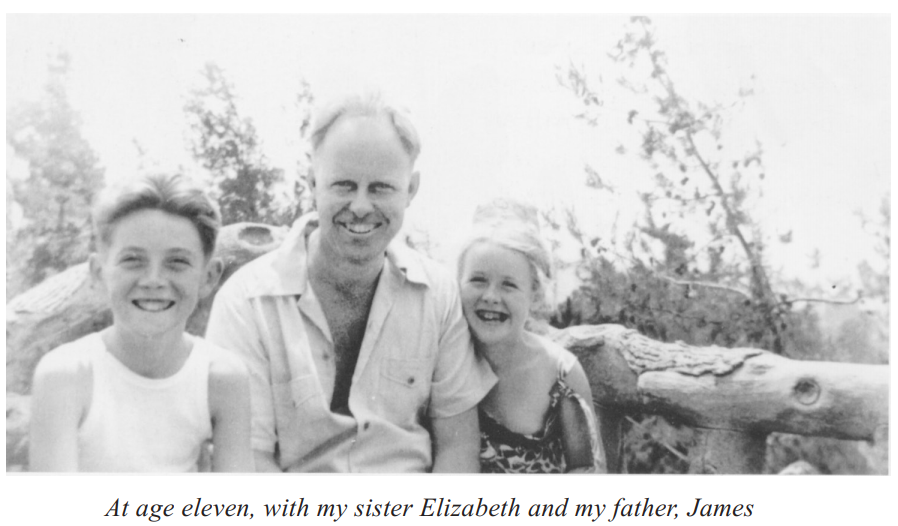
\includegraphics[width=0.75\linewidth]{image/Text5/Fig5.1.png}
\end{figure}

\noindent 4\\
The Hapsburgs added to their genetic woes by intermarrying. Arranging marriages between different branches of the Hapsburg clan and often among close relatives may have made political sense as a way of building alliances and ensuring dynastic succession, but it was anything but astute in genetic terms. Inbreeding of this kind can result in genetic disease, as the Hapsburgs found out to their cost. Charles II, the last of the Hapsburg monarchs in Spain, not only boasted a prize-worthy example of the family lip—he could not even chew his own food—but was also a complete invalid, and incapable, despite two marriages, of producing children.\\
哈布斯堡家族通过近亲结婚增加了他们的遗传问题。安排哈布斯堡家族不同分支之间,甚至经常是近亲之间的婚姻,可能在政治上有意义,作为建立联盟和确保王朝继承的一种方式,但在遗传学上却一点也不明智。这种近亲繁殖可能导致遗传疾病,哈布斯堡家族为此付出了代价。查理二世,西班牙哈布斯堡君主的最后一位,不仅拥有家族嘴唇的典型例子——他甚至不能咀嚼自己的食物——而且完全体弱多病,尽管有两次婚姻,却无法生育子女。\\

\noindent 5\\
Genetic disease has long stalked humanity. In some cases, such as Charles II’s, it has had a direct impact on history. Retrospective diagnosis has suggested that George III, the English king whose principal claim to fame is to have lost the American colonies in the Revolutionary War, suffered from an inherited disease, porphyria, which causes periodic bouts of madness. Some historians—mainly British ones—have argued that it was the distraction caused by George’s illness that permitted the Americans’ against-the-odds military success. While most hereditary diseases have no such geopolitical impact, they nevertheless have brutal and often tragic consequences for the afflicted families, sometimes for many generations. Understanding genetics is not just about understanding why we look like our parents. It is also about coming to grips with some of humankind’s oldest enemies: the flaws in our genes that cause genetic disease.\\
遗传病长期以来一直困扰着人类。在某些情况下,比如查理二世,它对历史产生了直接影响。回顾性诊断表明,乔治三世,这位以在独立战争中失去美国殖民地而闻名的英国国王,患有一种遗传病——卟啉症,这会导致周期性的疯狂发作。一些历史学家——主要是英国人——认为,正是乔治的疾病引起的分心,使得美国人取得了出人意料的军事成功。虽然大多数遗传病没有这样的地缘政治影响,但它们对受影响的家庭仍然有着残酷且往往悲惨的后果,有时甚至影响几代人。理解遗传学不仅仅是理解我们为什么长得像父母。它还涉及到与人类最古老的敌人之一——导致遗传病的基因缺陷——作斗争。\\

\noindent 6\\
Our ancestors must have wondered about the workings of heredity as soon as evolution endowed them with brains capable of formulating the right kind of question. And the readily observable principle that close relatives tend to be similar can carry you a long way if, like our ancestors, your concern with the application of genetics is limited to practical matters like improving domesticated animals (for, say, milk yield in cattle) and plants (for, say, the size of fruit). Generations of careful selection—breeding initially to domesticate appropriate species, and then breeding only from the most productive cows and from the trees with the largest fruit—resulted in animals and plants tailor-made for human purposes. Underlying this enormous unrecorded effort is that simple rule of thumb: that the most productive cows will produce highly productive offspring and from the seeds of trees with large fruit large-fruited trees will grow. Thus, despite the extraordinary advances of the past hundred years or so, the twentieth and twenty-first centuries by no means have a monopoly on genetic insight. Although it wasn’t until 1909 that the British biologist William Bateson gave the science of inheritance a name, genetics, and although the DNA revolution has opened up new and extraordinary vistas of potential progress, in fact the single greatest application of genetics to human well-being was carried out eons ago by anonymous ancient farmers. Almost everything we eat—cereals, fruit, meat, dairy products—is the legacy of that earliest and most far-reaching application of genetic manipulations to human problems.\\
我们的祖先一定在进化赋予他们能够提出正确问题的能力时,就对遗传的运作感到好奇。并且,近亲往往相似这一容易观察到的原则,如果像我们的祖先一样,你对遗传学的应用仅限于实际问题,如改善家养动物(例如,提高牛的产奶量)和植物(例如,增大水果的大小),那么这一原则可以带你走得很远。几代人的精心选择——最初是为了驯化合适的物种,然后只从产奶量最高的奶牛和果实最大的树上进行繁殖——结果产生了为人类目的量身定制的动物和植物。在这一巨大未记录的努力背后,是那条简单的经验法则:产奶量最高的奶牛将产生高生产力的后代,而从大果树木的种子中将生长出大果树木。因此,尽管在过去一百年左右的时间里取得了非凡的进步,但二十世纪和二十一世纪并不意味着对遗传学洞察力的垄断。尽管直到1909年,英国生物学家威廉·贝特森才给遗传学命名,尽管DNA革命开辟了新的、非凡的潜在进步视野,但实际上,对人类福祉的最大遗传学应用是由匿名的古代农民在很久以前进行的。我们吃的几乎所有东西——谷物、水果、肉类、乳制品——都是对人类问题最早和最深远的遗传操作应用的遗产。\\

\noindent 7\\
An understanding of the actual mechanics of genetics proved a tougher nut to crack. Gregor Mendel (1822–1884) published his famous paper on the subject in 1866 (and it was ignored by the scientific community for another thirty-four years). Why did it take so long? After all, heredity is a major aspect of the natural world, and, more important, it is readily, and universally, observable: a dog owner sees how a cross between a brown and black dog turns out, and all parents consciously or subconsciously track the appearance of their own characteristics in their children. One simple reason is that genetic mechanisms turn out to be complicated. Mendel’s solution to the problem is not intuitively obvious: children are not, after all, simply a blend of their parents’ characteristics. Perhaps most important was the failure by early biologists to distinguish between two fundamentally different processes, heredity and development. Today we understand that a fertilized egg contains the genetic information, contributed by both parents, that determines whether someone will be afflicted with, say, porphyria. That is heredity. The subsequent process, the development of a new individual from that humble starting point of a single cell, the fertilized egg, involves implementing that information. Broken down in terms of academic disciplines, genetics focuses on the information and developmental biology focuses on the use of that information. Lumping heredity and development together into a single phenomenon, early scientists never asked the questions that might have steered them toward the secret of heredity. Nevertheless, the effort had been under way in some form since the dawn of Western history.\\
对遗传学实际机制的理解证明是一个更难破解的难题。格雷戈尔·孟德尔(1822-1884)在1866年发表了他关于这个主题的著名论文(但科学界又忽视了另外三十四年)。为什么花了这么长时间?毕竟,遗传是自然界的一个主要方面,而且更重要的是,它是容易和普遍可观察的:狗的主人可以看到棕色和黑色狗的杂交结果,所有的父母都会有意或无意地追踪自己特征在孩子身上的表现。一个简单的原因是遗传机制结果很复杂。孟德尔对这个问题的解决方案并不直观明显:毕竟,孩子们并不是简单地混合了他们父母的特征。也许最重要的是早期生物学家未能区分两个根本不同的过程,遗传和发育。今天我们知道,受精卵包含了双方父母贡献的遗传信息,这些信息决定了某人是否会患有例如卟啉症。这就是遗传。随后的过程,即从单个细胞——受精卵这一谦卑的起点发展成一个新的个体,涉及实施这些信息。从学术学科的角度来看,遗传学专注于信息,而发育生物学专注于使用这些信息。将遗传和发育合并为一个单一现象,早期科学家从未提出可能引导他们揭开遗传秘密的问题。然而,这种努力自西方历史黎明以来就以某种形式进行着。\\

\noindent 8\\
The Greeks, including Hippocrates, pondered heredity. They devised a theory of “pangenesis,” which claimed that sex involved the transfer of miniaturized body parts: “Hairs, nails, veins, arteries, tendons and their bones, albeit invisible as their particles are so small. While growing, they gradually separate from each other.” This idea enjoyed a brief renaissance when Charles Darwin, desperate to support his theory of evolution by natural selection with a viable hypothesis of inheritance, put forward a modified version of pangenesis in the second half of the nineteenth century. In Darwin’s scheme, each organ—eyes, kidneys, bones—contributed circulating “gemmules” that accumulated in the sex organs, and were ultimately exchanged in the course of sexual reproduction. Because these gemmules were produced throughout an organism’s lifetime, Darwin argued any change that occurred in the individual after birth, like the stretch of a giraffe’s neck imparted by craning for the highest foliage, could be passed on to the next generation. Ironically, then, to buttress his theory of natural selection Darwin came to champion aspects of Jean-Baptiste Lamarck’s theory of inheritance of acquired characteristics—the very theory that his evolutionary ideas did so much to discredit. Darwin was invoking only Lamarck’s theory of inheritance; he continued to believe that natural selection was the driving force behind evolution, but supposed that natural selection operated on the variation produced by pangenesis. Had Darwin known about Mendel’s work (although Mendel published his results shortly after The Origin of Species appeared, Darwin was never aware of them), he might have been spared the embarrassment of this late-career endorsement of some of Lamarck’s ideas.\\
希腊人,包括希波克拉底,思考过遗传问题。他们提出了一种“泛生论”理论,声称性行为涉及微小化身体部位的转移:“头发、指甲、静脉、动脉、肌腱及其骨骼,尽管它们的颗粒非常小而看不见。在生长过程中,它们逐渐彼此分离。”当查尔斯·达尔文迫切希望用一个可行的遗传假设来支持他的自然选择进化论时,这个想法在十九世纪下半叶经历了短暂的复兴。在达尔文的方案中,每个器官——眼睛、肾脏、骨骼——都贡献了循环的“芽球”,这些芽球在性器官中积累,并最终在性繁殖过程中交换。由于这些芽球是在生物体的一生中产生的,达尔文认为任何在出生后发生的个体变化,如长颈鹿为了获取最高处的树叶而伸长脖子,都可以传递给下一代。具有讽刺意味的是,为了支持他的自然选择理论,达尔文开始支持让-巴蒂斯特·拉马克的获得性遗传特征理论的某些方面——正是他的进化思想极大地贬低了这一理论。达尔文只引用了拉马克的遗传理论;他继续相信自然选择是进化背后的驱动力,但认为自然选择作用于泛生论产生的变异。如果达尔文知道孟德尔的工作(尽管孟德尔在《物种起源》发表后不久就发表了他的结果,但达尔文从未了解过),他可能就不会因为晚年支持拉马克的一些观点而感到尴尬了。\\

\noindent 9\\
Whereas pangenesis supposed that embryos were assembled from a set of minuscule components, another approach, “preformationism,” avoided the assembly step altogether: either the egg or the sperm (exactly which was a contentious issue) contained a complete preformed individual called a homunculus. Development was therefore merely a matter of enlarging this into a fully formed being. In the days of preformationism, what we now recognize as genetic disease was variously interpreted: sometimes as a manifestation of the wrath of God or the mischief of demons and devils; sometimes as evidence of either an excess of or a deficit of the father’s “seed”; sometimes as the result of “wicked thoughts” on the part of the mother during pregnancy. On the premise that fetal malformation can result when a pregnant mother’s desires are thwarted, leaving her feeling stressed and frustrated, Napoleon passed a law permitting expectant mothers to shoplift. None of these notions, needless to say, did much to advance our understanding of genetic disease.\\
与泛生论认为胚胎是由一组微小的组成部分组装而成的不同,另一种方法“预成论”完全避免了组装步骤:无论是卵子还是精子(具体是哪一个是有争议的问题)都包含一个完整的预成个体,称为侏儒。因此,发育仅仅是将这个个体扩大成一个完全形成的生物体。在预成论的时代,我们现在所认识的遗传病被以各种方式解释:有时被认为是上帝的愤怒或恶魔和魔鬼的恶作剧的表现;有时被认为是父亲“种子”过多或不足的证据;有时被认为是母亲在怀孕期间“邪恶思想”的结果。基于孕妇的欲望受挫,感到压力和沮丧时可能导致胎儿畸形的前提,拿破仑通过了一项法律,允许孕妇偷窃。不用说,这些观点都没有对我们理解遗传病做出太多贡献。\\

\noindent 10\\
By the early nineteenth century, better microscopes had defeated preformationism. Look as hard as you like, you will never see a tiny homunculus curled up inside a sperm or egg cell. Pangenesis, though an earlier misconception, lasted rather longer—the argument would persist that the gemmules were simply too small to visualize—but was eventually laid to rest by August Weismann, who argued that inheritance depended on the continuity of germ plasm between generations and thus changes to the body over an individual's lifetime could not be transmitted to subsequent generations. His simple experiment involved cutting the tails off several generations of mice. According to Darwin's pangenesis, tailless mice would produce gemmules signifying "no tail" and so their offspring should develop a severely stunted hind appendage or none at all. When Weismann showed that the tail kept appearing after many generations of amputees, pangenesis bit the dust.\\
到了十九世纪初,更好的显微镜已经击败了预成论。无论你怎么努力看,你都不会在精子或卵细胞内看到一个蜷缩的小侏儒。泛生论虽然是一个早期的误解,但持续时间较长——争论会持续认为芽球太小而无法观察到——但最终被奥古斯特·魏斯曼平息,他认为遗传依赖于代际之间生殖质的连续性,因此个体一生中的身体变化不能传递给后代。他的简单实验包括切断几代老鼠的尾巴。根据达尔文的泛生论,无尾老鼠会产生表示“无尾”的芽球,因此它们的后代应该发育出严重发育不良的后肢或根本没有后肢。当魏斯曼表明即使在许多代截肢者之后尾巴仍然出现时,泛生论寿终正寝。\\

\begin{figure}
    \centering
    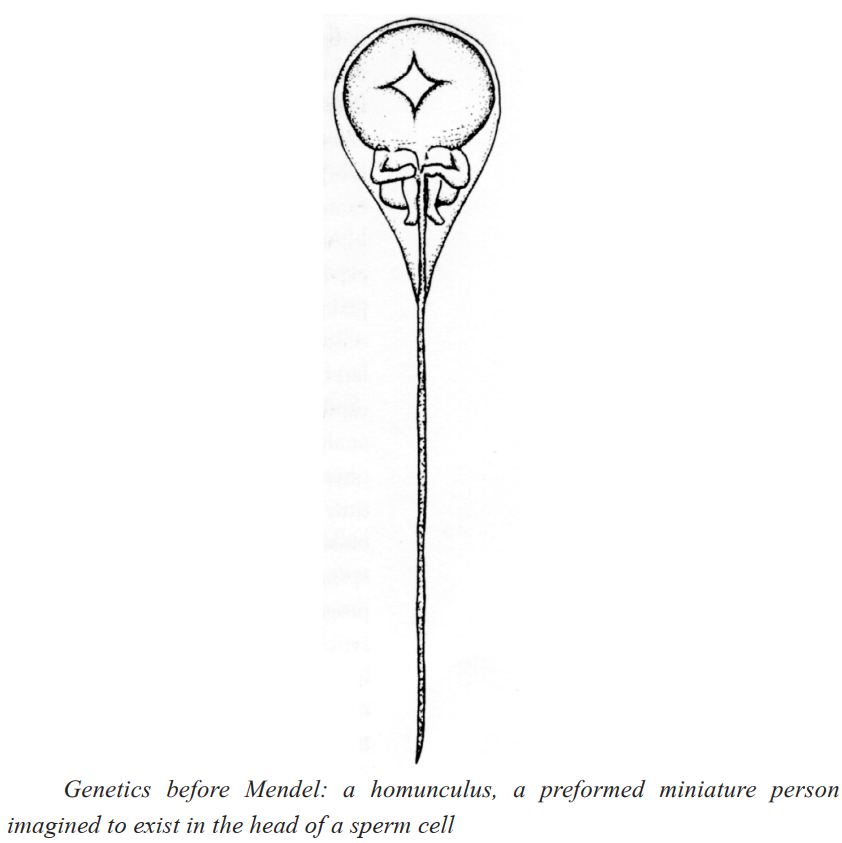
\includegraphics[width=0.75\linewidth]{image/Text5/Fig5.2.png}
\end{figure}

\noindent 11\\
Gregor Mendel was the one who got it right. By any standards, however, he was an unlikely candidate for scientific superstardom. Born to a farming family in what is now the Czech Republic, he excelled at the village school and, at twenty-one, entered the Augustinian monastery at Brünn. After proving a disaster as a parish priest—his response to the ministry was a nervous breakdown—he tried his hand at teaching. By all accounts he was a good teacher, but in order to qualify to teach a full range of subjects, he had to take an exam. He failed it. Mendel’s father superior, Abbot Napp, then dispatched him to the University of Vienna, where he was to bone up full-time for the retesting. Despite apparently doing well in physics at Vienna, Mendel again failed the exam, and so never rose above the rank of substitute teacher.\\
格雷戈尔·孟德尔是那个做对的人。然而,按照任何标准,他都是一个不太可能成为科学超级巨星的候选人。他出生在现在捷克共和国的一个农民家庭,在乡村学校表现出色,二十一岁时进入了布尔诺的奥古斯丁修道院。在证明作为教区牧师是个灾难后——他对牧师职务的反应是精神崩溃——他尝试了教学。据大家说,他是一位好老师,但为了有资格教授全部科目,他必须参加考试。他没有通过。孟德尔的上级,纳普修道院长,随后派他去维也纳大学,在那里他要全职准备重新考试。尽管在维也纳物理学似乎学得很好,孟德尔再次考试失败,因此从未超过代课教师的职位。\\

\noindent 12\\
Around 1856, at Abbot Napp's suggestion, Mendel undertook some scientific experiments on heredity. He chose to study a number of characteristics of the pea plants he grew in his own patch of the monastery garden. In 1865 he presented his results to the local natural history society in two lectures, and, a year later, published them in the society's journal. The work was a tour de force: the experiments were brilliantly designed and painstakingly executed, and his analysis of the results was insightful and deft. It seems that his training in physics contributed to his breakthrough because, unlike other biologists of that time, he approached the problem quantitatively. Rather than simply noting that crossbreeding of red and white flowers resulted in some red and some white offspring, Mendel actually counted them, realizing that the ratios of red to white progeny might be significant—as indeed they are. Despite sending copies of his article to various prominent scientists, Mendel found himself completely ignored by the scientific community. His attempt to draw attention to his results merely backfired. He wrote to his one contact among the ranking scientists of the day, botanist Karl Nägeli in Munich, asking him to replicate the experiments, and he duly sent off 140 carefully labeled packets of seeds. He should not have bothered. Nägeli believed that the obscure monk should be of service to him, rather than the other way around, so he sent Mendel seeds of his own favorite plant, hawkweed, challenging the monk to re-create his results with a different species. Sad to say, for various reasons, hawkweed is not well-suited to breeding experiments such as those Mendel had performed on the peas. The entire exercise was a waste of his time.\\
大约在1856年,在纳普修道院长的建议下,孟德尔进行了一些关于遗传的科学实验。他选择研究他在修道院花园里自己种植的豌豆植物的一些特性。1865年,他在当地自然历史学会的两次讲座中展示了他的结果,一年后,他将这些结果发表在学会的期刊上。这项工作是一次杰作:实验设计巧妙,执行精心,他对结果的分析富有洞察力和技巧。看来他在物理学方面的训练促成了他的突破,因为与其他当时的生物学家不同,他量化地处理了这个问题。孟德尔并没有简单地注意到红花和白花的杂交产生了一些红花和一些白花的后代,而是实际进行了计数,意识到红白后代的比例可能很重要——实际上确实如此。尽管他将文章的副本寄给了多位著名科学家,孟德尔发现自己完全被科学界忽视。他试图引起人们对他结果的关注,但只是适得其反。他写信给他那个时代排名靠前的科学家之一,慕尼黑的植物学家卡尔·纳格利,请求他复制实验,他也确实寄出了140包仔细标记的种子。他本不应该费心。纳格利认为这位默默无闻的修士应该为他服务,而不是反过来,所以他给孟德尔寄去了他自己最喜欢的植物——鹰爪草的种子,挑战这位修士用不同的物种重现他的结果。遗憾的是,由于各种原因,鹰爪草并不适合进行孟德尔在豌豆上进行的那种繁殖实验。整个练习都是浪费时间。\\

\noindent 13\\
Mendel’s low-profile existence as monk-teacher-researcher ended abruptly in 1868 when, on Napp’s death, he was elected abbot of the monastery. Although he continued his research—increasingly on bees and the weather—administrative duties were a burden, especially as the monastery became embroiled in a messy dispute over back taxes. Other factors, too, hampered him as a scientist. Portliness eventually curtailed his fieldwork: as he wrote, hill climbing had become “very difficult for me in a world where universal gravitation prevails.” His doctors prescribed tobacco to keep his weight in check, and he obliged them by smoking twenty cigars a day, as many as Winston Churchill. It was not his lungs, however, that let him down: in 1884, at the age of sixty-one, Mendel succumbed to a combination of heart and kidney disease.\\
孟德尔作为修士、教师和研究者的低调生活因纳普去世而在1868年突然结束,他被选为修道院的院长。尽管他继续他的研究——越来越多地涉及蜜蜂和天气——但行政职责成为了负担,特别是当修道院卷入了一场关于欠税的混乱纠纷时。其他因素也阻碍了他作为科学家的工作。最终,肥胖限制了他的实地工作:正如他所写,在普遍引力盛行的世界中,爬山对我来说变得“非常困难”。他的医生开处方让他吸烟以控制体重,他遵从医嘱每天吸二十支雪茄,和温斯顿·丘吉尔一样多。然而,让他倒下的不是他的肺:1884年,61岁的孟德尔因心脏和肾脏疾病去世。\\

\noindent 14\\
Not only were Mendel’s results buried in an obscure journal, but they would have been unintelligible to most scientists of the era. He was far ahead of his time with his combination of careful experiment and sophisticated quantitative analysis. Little wonder, perhaps, that it was not until 1900 that the scientific community caught up with him. The rediscovery of Mendel’s work, by three plant geneticists interested in similar problems, provoked a revolution in biology. At last the scientific world was ready for the monk’s peas.\\
孟德尔的结果不仅被埋没在一个鲜为人知的期刊中,而且对那个时代的大多数科学家来说是无法理解的。他以其精心的实验和复杂的定量分析远远超前于他的时代。也许不足为奇的是,直到1900年科学界才赶上他。三位对类似问题感兴趣的植物遗传学家重新发现了孟德尔的工作,引发了生物学领域的一场革命。终于,科学界准备好接受这位修道士的豌豆了。\\

\noindent 15\\
Mendel realized that there are specific factors—later to be called “genes”—that are passed from parent to offspring. He worked out that these factors come in pairs and that the offspring receives one from each parent.\\
孟德尔意识到有一些特定的因素——后来被称为“基因”——是从父母传给后代的。他推算出这些因素是成对出现的,后代从每个父母那里各继承一个。\\

\noindent 16\\
Noticing that peas came in two distinct colors, green and yellow, he deduced that there were two versions of the pea-color gene. A pea has to have two copies of the G version if it is to become green, in which case we say that it is GG for the pea-color gene. It must therefore have received a G pea-color gene from both of its parents. However, yellow peas can result both from YY and YG combinations. Having only one copy of the Y version is sufficient to produce yellow peas. Y trumps G. Because in the YG case the Y signal dominates the G signal, we call Y “dominant.” The subordinate G version of the pea-color gene is called “recessive.”\\
他注意到豌豆有两种明显的颜色,绿色和黄色,他推断豌豆颜色基因有两个版本。如果豌豆要变成绿色,它必须有两个G版本的副本,我们称其为豌豆颜色基因的GG。因此,它必须从两个父母那里各获得一个G颜色基因。然而,黄色豌豆可以由YY和YG组合产生。只要有一个Y版本的副本就足以产生黄色豌豆。Y优于G。因为在YG的情况下,Y信号支配G信号,我们称Y为“显性”。从属的G版本的豌豆颜色基因被称为“隐性”。\\

\noindent 17\\
Each parent pea plant has two copies of the pea-color gene, yet it contributes only one copy to each offspring; the other copy is furnished by the other parent. In plants, pollen grains contain sperm cells—the male contribution to the next generation—and each sperm cell contains just one copy of the pea-color gene. A parent pea plant with a YG combination will produce sperm that contain either a Y version or a G one. Mendel discovered that the process is random: 50 percent of the sperm produced by that plant will have a Y and 50 percent will have a G.\\
每个亲本豌豆植物都有两个豌豆颜色基因的副本,但它只向每个后代贡献一个副本;另一个副本由另一个亲本提供。在植物中,花粉粒包含精子细胞——对下一代的雄性贡献——每个精子细胞只包含一个豌豆颜色基因的副本。具有YG组合的亲本豌豆植物将产生包含Y版本或G版本的精子。孟德尔发现这个过程是随机的:该植物产生的精子中有50\%带有Y,50\%带有G。\\

\noindent 18\\
Suddenly many of the mysteries of heredity made sense. Characteristics, like the Hapsburg Lip, that are transmitted with a high probability (actually 50 percent) from generation to generation are dominant. Other characteristics that appear in family trees much more sporadically, often skipping generations, may be recessive. When a gene is recessive an individual has to have two copies of it for the corresponding trait to be expressed. Those with one copy of the gene are carriers: they don’t themselves exhibit the characteristic, but they can pass the gene on. Albinism, in which the body fails to produce pigment so the skin and hair are strikingly white, is an example of a recessive characteristic that is transmitted in this way. Therefore, to be albino you have to have two copies of the gene, one from each parent. (This was the case with the Reverend Dr. William Archibald Spooner, who was also—perhaps only by coincidence—prone to a peculiar form of linguistic confusion whereby, for example, “a well-oiled bicycle” might become “a well-boiled icicle.” Such reversals would come to be termed “spoonerisms” in his honor.) Your parents, meanwhile, may have shown no sign of the gene at all. If, as is often the case, each has only one copy, then they are both carriers. The trait has skipped at least one generation.\\
突然间,许多遗传的奥秘变得有意义了。像哈布斯堡唇这样以高概率(实际上是50\%)代代相传的特征是显性的。其他在家族树中更零星出现的特征,经常跳过几代,可能是隐性的。当一个基因是隐性的时,个体必须拥有两个副本才能表现出相应的特征。拥有一个基因副本的人是携带者:他们自己不表现出特征,但可以传递基因。白化病,即身体无法产生色素,导致皮肤和头发异常白皙,就是这样一种隐性特征的例子。因此,要成为白化病患者,你必须拥有两个基因副本,每个父母各提供一个。(这与威廉·阿奇博尔德·斯波纳牧师的情况相同,他也可能只是巧合地容易犯一种特殊的语言混淆错误,例如,“a well-oiled bicycle”可能会变成“a well-boiled icicle”。这种颠倒会以他的名字被称为“斯波纳现象”。)与此同时,你的父母可能根本没有表现出基因的迹象。如果情况经常是这样,每个父母只有一个副本,那么他们都是携带者。该特征至少跳过了一代。\\

\noindent 19\\
Mendel’s results implied that things—material objects—were transmitted from generation to generation. But what was the nature of these things?\\
孟德尔的结果暗示了一些东西——物质对象——是从一代传给下一代的。但这些东西的本质是什么?\\

\noindent 20\\
At about the time of Mendel’s death in 1884, scientists using ever-improving optics to study the minute architecture of cells coined the term “chromosome” to describe the long stringy bodies in the cell nucleus. But it was not until 1902 that Mendel and chromosomes came together.\\
大约在孟德尔1884年去世时,科学家们使用不断改进的光学技术研究细胞的微观结构,并创造了“染色体”一词来描述细胞核中的长丝状体。但直到1902年,孟德尔和染色体才联系在一起。\\

\begin{figure}
    \centering
    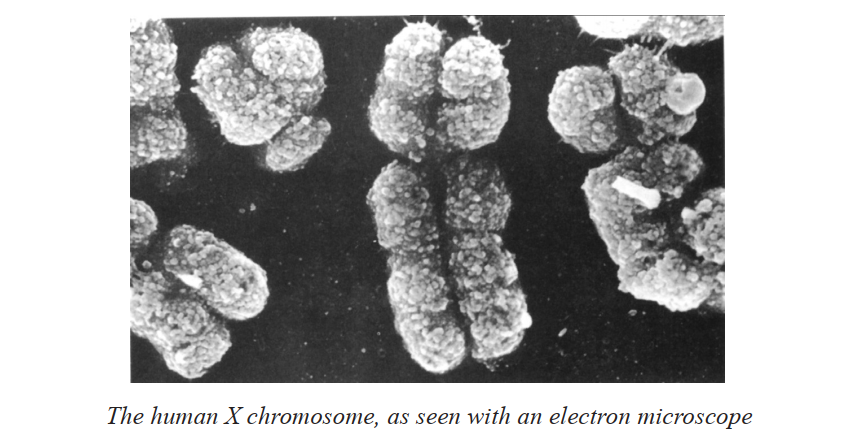
\includegraphics[width=0.75\linewidth]{image/Text5/Fig5.3.png}
\end{figure}

\noindent 21\\
A medical student at Columbia University, Walter Sutton, realized that chromosomes had a lot in common with Mendel’s mysterious factors. Studying grasshopper chromosomes, Sutton noticed that most of the time they are doubled up—just like Mendel’s paired factors. But Sutton also identified one type of cell in which chromosomes were not paired: the sex cells. Grasshopper sperm have only a single set of chromosomes, not a double set. This was exactly what Mendel had described: his pea plant sperm cells also only carried a single copy of each of his factors. It was clear that Mendel’s factors, now called genes, must be on the chromosomes.\\
哥伦比亚大学的一名医学生沃尔特·萨顿意识到染色体与孟德尔的神秘因素有很多共同之处。研究蚱蜢的染色体时,萨顿注意到大多数时候它们是成对出现的——就像孟德尔的配对因素一样。但萨顿也发现了一种染色体不成对的细胞类型:性细胞。蚱蜢精子只有一套染色体,而不是两套。这正是孟德尔所描述的:他的豌豆植物精子细胞也只携带每个因素的一个副本。很明显,孟德尔的因素,现在被称为基因,一定位于染色体上。\\

\noindent 22\\
In Germany Theodor Boveri independently came to the same conclusions as Sutton, and so the biological revolution their work had precipitated came to be called the Sutton-Boveri chromosome theory of inheritance. Suddenly genes were real. They were on chromosomes, and you could actually see chromosomes through the microscope.\\
在德国,西奥多·博韦里独立地得出了与萨顿相同的结论,因此他们工作引发的生物学革命被称为萨顿-博韦里染色体遗传理论。突然间,基因变得真实存在。它们位于染色体上,你实际上可以通过显微镜看到染色体。\\

\noindent 23\\
Not everyone bought the Sutton-Boveri theory. One skeptic was Thomas Hunt Morgan, also at Columbia. Looking down the microscope at those stringy chromosomes, he could not see how they could account for all the changes that occur from one generation to the next. If all the genes were arranged along chromosomes, and all chromosomes were transmitted intact from one generation to the next, then surely many characteristics would be inherited together. But since empirical evidence showed this not to be the case, the chromosomal theory seemed insufficient to explain the variation observed in nature. Being an astute experimentalist, however, Morgan had an idea how he might resolve such discrepancies. He turned to the fruit fly, Drosophila melanogaster, the drab little beast that, ever since Morgan, has been so beloved by geneticists.\\
并不是每个人都接受萨顿-博韦里理论。一位怀疑论者是哥伦比亚大学的托马斯·亨特·摩根。通过显微镜观察那些细长的染色体,他无法理解它们如何解释一代代之间发生的变化。如果所有的基因都排列在染色体上,并且所有染色体都完整地从一代传给下一代,那么许多特征肯定会一起遗传。但由于经验证据表明事实并非如此,染色体理论似乎不足以解释自然界中观察到的变异。然而,作为一个敏锐的实验家,摩根有了一个解决这些差异的想法。他转向了果蝇,黑腹果蝇,这种不起眼的小生物,自从摩根以来,一直受到遗传学家的喜爱。\\

\begin{figure}
    \centering
    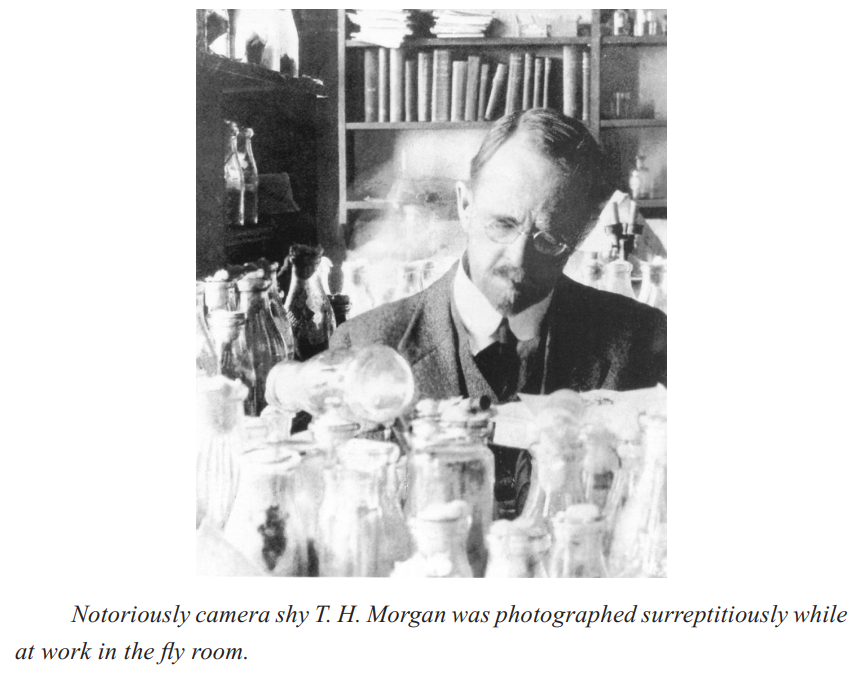
\includegraphics[width=0.75\linewidth]{image/Text5/Fig5.4.png}
\end{figure}

\noindent 24\\
In fact, Morgan was not the first to use the fruit fly in breeding experiments—that distinction belonged to a lab at Harvard that first put the critter to work in 1901—but it was Morgan’s work that put the fly on the scientific map. Drosophila is a good choice for genetic experiments. It is easy to find (as anyone who has left out a bunch of overripe bananas during the summer well knows); it is easy to raise (bananas will do as feed); and you can accommodate hundreds of flies in a single milk bottle (Morgan’s students had no difficulty acquiring milk bottles, pinching them at dawn from doorsteps in their Manhattan neighborhood); and it breeds and breeds (a whole generation takes about ten days, and each female lays several hundred eggs). Starting in 1907 in a famously squalid, cockroach-infested, banana-stinking lab that came to be known affectionately as the “fly room,” Morgan and his students (“Morgan’s boys” as they were called) set to work on fruit flies.\\
事实上,摩根并不是第一个在育种实验中使用果蝇的人——这一荣誉属于1901年首次让果蝇工作的哈佛大学实验室——但正是摩根的工作让果蝇在科学界声名鹊起。果蝇是遗传实验的好选择。它很容易找到(任何在夏天留下一堆过熟香蕉的人都知道);它很容易饲养(香蕉可以作为食物);你可以在一只牛奶瓶中容纳数百只果蝇(摩根的学生在曼哈顿的家门口轻松地获取牛奶瓶);而且它繁殖迅速(整个一代大约需要十天,每只雌性产下数百个卵)。从1907年开始,在一个以肮脏、蟑螂成灾、香蕉味弥漫而闻名的实验室里,这个实验室后来被亲切地称为“果蝇室”,摩根和他的学生们(他们被称为“摩根的男孩”)开始研究果蝇。\\

\noindent 25\\
Unlike Mendel, who could rely on the variant strains isolated over the years by farmers and gardeners—yellow peas as opposed to green ones, wrinkled skin as opposed to smooth—Morgan had no menu of established genetic differences in the fruit fly to draw upon. And you cannot do genetics until you have isolated some distinct characteristics to track through the generations. Morgan’s first goal therefore was to find “mutants,” the fruit fly equivalents of yellow or wrinkled peas. He was looking for genetic novelties, random variations that somehow simply appeared in the population.\\
与孟德尔不同,孟德尔可以依靠农民和园丁多年来分离出的变种——黄色豌豆与绿色豌豆相对,皱皮与光滑皮相对——摩根没有现成的果蝇遗传差异菜单可供参考。而且在你隔离出一些可以追踪几代的明显特征之前,你无法进行遗传学研究。因此,摩根的第一个目标是找到“突变体”,即果蝇中的黄色或皱皮豌豆的等价物。他正在寻找遗传新奇性,即随机变异,这些变异不知何故地出现在种群中。\\

\noindent 26\\
One of the first mutants Morgan observed turned out to be one of the most instructive. While normal fruit flies have red eyes, these had white ones. And he noticed that the white-eyed flies were typically male. It was known that the sex of a fruit fly—or, for that matter, the sex of a human—is determined chromosomally: females have two copies of the X chromosome, whereas males have one copy of the X and one copy of the much smaller Y. In light of this information, the white-eye result suddenly made sense: the eye-color gene is located on the X chromosome and the white-eye mutation, W, is recessive. Because males have only a single X chromosome, even recessive genes, in the absence of a dominant counterpart to suppress them, are automatically expressed. White-eyed females were relatively rare because they typically had only one copy of W so they expressed the dominant red eye color. By correlating a gene—the one for eye color—with a chromosome, the X, Morgan, despite his initial reservations, had effectively proved the Sutton-Boveri theory. He had also found an example of “sex-linkage,” in which a particular characteristic is disproportionately represented in one sex.\\
摩根观察到的第一个突变体之一结果是最有启发性的。正常的果蝇有红色的眼睛,而这些果蝇有白色的眼睛。他注意到白眼果蝇通常是雄性。已知果蝇或人类的性别是由染色体决定的:雌性有两个X染色体的副本,而雄性有一个X和一个较小的Y。根据这些信息,白眼结果突然变得有意义:眼色基因位于X染色体上,白眼突变W是隐性的。因为雄性只有一个X染色体,即使是隐性基因,在没有显性对应基因来抑制它们的情况下,也会自动表现出来。白眼雌性相对较少,因为它们通常只有一个W副本,所以表现出显性的红色眼睛。通过将一个基因——眼色基因——与X染色体相关联,摩根尽管最初有所保留,但有效地证明了萨顿-博韦里理论。他还发现了一个“性连锁”的例子,其中一个特定特征在一个性别中不成比例地表现出来。\\

\noindent 27\\
Like Morgan’s fruit flies, Queen Victoria provides a famous example of sex-linkage. On one of her X chromosomes, she had a mutated gene for hemophilia, the “bleeding disease” in whose victims proper blood clotting fails to occur. Because her other copy was normal, and the hemophilia gene is recessive, she herself did not have the disease. But she was a carrier. Her daughters did not have the disease either; evidently each possessed at least one copy of the normal version. But Victoria’s sons were not all so lucky. Like all males (fruit fly males included), each had only one X chromosome; this was necessarily derived from Victoria (a Y chromosome could have come only from Prince Albert, Victoria’s husband). Because Victoria had one mutated copy and one normal copy, each of her sons had a 50-50 chance of having the disease. Prince Leopold drew the short straw: he developed hemophilia, and died at thirty-one, bleeding to death after a minor fall. Two of Victoria’s daughters, Princesses Alice and Beatrice, were carriers, having inherited the mutated gene from their mother. They each produced carrier daughters and sons with hemophilia. Alice’s grandson Alexis, heir to the Russian throne, had hemophilia, and would doubtless have died young had the Bolsheviks not gotten to him first.\\
像摩根的果蝇一样,维多利亚女王提供了性连锁的一个著名例子。在她的一条X染色体上,她有一个血友病的突变基因,这是一种“出血病”,患者的正常凝血无法发生。因为她的另一个副本是正常的,而且血友病基因是隐性的,她自己并没有这种疾病。但她是一个携带者。她的女儿们也没有这种疾病;显然每人至少拥有一个正常版本的副本。但维多利亚的儿子们并不都那么幸运。像所有雄性(包括果蝇雄性)一样,他们每人只有一个X染色体;这必然来自维多利亚(Y染色体只能来自维多利亚的丈夫阿尔伯特亲王)。因为维多利亚有一个突变副本和一个正常副本,她的每个儿子都有50-50的几率患病。利奥波德王子不幸中招:他患了血友病,在一次轻微摔倒后因出血过多而死,年仅31岁。维多利亚的两个女儿,爱丽丝公主和比阿特丽斯公主,是携带者,她们从母亲那里继承了突变基因。她们各自生下了携带者女儿和患有血友病的儿子。爱丽丝的孙子,俄罗斯王位继承人阿列克谢,患有血友病,如果不是布尔什维克人先找到他,他无疑会早逝。\\

\noindent 28\\
Morgan's fruit flies had other secrets to reveal. In the course of studying genes located on the same chromosome, Morgan and his students found that chromosomes actually break apart and re-form during the production of sperm and egg cells. This meant that Morgan's original objections to the Sutton-Boveri theory were unwarranted: the breaking and re-forming—“recombination,” in modern genetic parlance—shuffles gene copies between members of a chromosome pair. This means that, say, the copy of chromosome 12 I got from my mother (the other, of course, comes from my father) is in fact a mix of my mother’s two copies of chromosome 12, one of which came from her mother and one from her father. Her two 12s recombined—exchanged material—during the production of the egg cell that eventually turned into me. Thus my maternally derived chromosome 12 can be viewed as a mosaic of my grandparents’ 12s. Of course, my mother's maternally derived 12 was itself a mosaic of her grandparents’ 12s, and so on.\\
摩根的果蝇还有其他秘密要揭示。在研究位于同一染色体上的基因的过程中,摩根和他的学生发现染色体实际上在精子和卵细胞的生产过程中会分离并重新形成。这意味着摩根对萨顿-博韦里理论的最初反对是没有根据的:现代遗传学中所说的“重组”——即在染色体对成员之间洗牌基因副本——是成立的。这意味着,比如说,我从母亲那里得到的第12号染色体的副本实际上是我母亲两个第12号染色体副本的混合,其中一个来自她的母亲的,一个来自她的父亲。她的两个第12号染色体在形成最终变成我的卵细胞过程中重新组合——交换了物质。因此,我母亲遗传给我的第12号染色体可以看作是我祖父母的第12号染色体的马赛克。当然,我母亲从她母亲那里遗传的第12号染色体本身也是她祖父母的第12号染色体的马赛克,以此类推。\\

\noindent 29\\
Recombination permitted Morgan and his students to map out the positions of particular genes along a given chromosome. Recombination involves breaking (and re-forming) chromosomes. Because genes are arranged like beads along a chromosome string, a break is statistically much more likely to occur between two genes that are far apart (with more potential break points intervening) on the chromosome than between two genes that are close together. If, therefore, we see a lot of reshuffling for any two genes on a single chromosome, we can conclude that they are a long way apart; the rarer the reshuffling, the closer the genes likely are. This basic and immensely powerful principle underlies all of genetic mapping. One of the primary tools of scientists involved in the Human Genome Project and of researchers at the forefront of the battle against genetic disease was thus developed all those years ago in the filthy, cluttered Columbia fly room. Each new headline in the science section of the newspaper these days along the lines of “Gene for Something Located” is a tribute to the pioneering work of Morgan and his boys.\\
重组使摩根和他的学生能够绘制出特定基因在给定染色体上的位置。重组涉及断裂(和重新形成)染色体。由于基因像珠子一样排列在染色体串上,断裂在统计上更有可能发生在染色体上相距较远的两个基因之间(有更多的潜在断裂点),而不是发生在相距较近的两个基因之间。因此,如果在单个染色体上的任意两个基因之间我们看到了大量的重组,我们可以得出结论,它们相距很远;重组越少,基因可能越近。这一基本而强大的原则支撑着所有的基因图谱系。参与人类基因组计划的科学家和在与遗传病作斗争的研究人员的主要工具之一,就是多年前在杂乱的哥伦比亚果蝇室中开发的。如今报纸科学版上的每一个“基因定位于某物”的新标题都是对摩根和他的学生们开创性工作的致敬。\\

\noindent 30\\
The rediscovery of Mendel’s work, and the breakthroughs that followed it, sparked a surge of interest in the social significance of genetics. While scientists had been grappling with the precise mechanisms of heredity through the eighteenth and nineteenth centuries, public concern had been mounting about the burden placed on society by what came to be called the “degenerate classes”—the inhabitants of poorhouses, workhouses, and insane asylums. What could be done with these people? It remained a matter of controversy whether they should be treated charitably—which, the less charitably inclined claimed, ensured such folk would never exert themselves and would therefore remain forever dependent on the largesse of the state or of private institutions—or whether they should be simply ignored, which, according to the charitably inclined, would result only in perpetuating the inability of the unfortunate to extricate themselves from their blighted circumstances.\\
孟德尔工作的重新发现以及随之而来的突破,引发了人们对遗传学社会意义的兴趣激增。虽然科学家们一直在努力解决十八和十九世纪遗传的精确机制,公众对所谓的“退化阶级”——贫民窟、济贫民院和精神病院的居民——给社会带来的负担感到担忧。应该如何处理这些人?他们是否应该得到慈善对待——不那么慈善的人声称,这确保了这些人永远不会努力,因此将永远依赖国家或私人机构的慷慨——还是应该被忽视,根据慈善倾向的人说,这只会使不幸者无法摆脱他们悲惨的处境遇。\\

\noindent 31\\
The publication of Darwin’s Origin of Species in 1859 brought these issues into sharp focus. Although Darwin carefully omitted to mention human evolution, fearing that to do so would only further inflame an already raging controversy, it required no great leap of imagination to apply his idea of natural selection to humans. Natural selection is the force that determines the fate of all genetic variations in nature—mutations like the one Morgan found in the fruit fly eye-color gene, but also perhaps differences in the abilities of human individuals to fend for themselves.\\
达尔文的《物种起源》在1859年出版,使这些问题成为焦点。尽管达尔文小心翼翼地避免提及人类进化,担心这样做只会进一步激化已经激烈的争议,但将他的自然选择理论应用于人类并不需要很大的想象力。自然选择是决定自然界所有遗传变异命运的力量——像摩根在果蝇眼色基因中发现的突变,但也许还有人类个体自卫能力的差异。\\

\noindent 32\\
Natural populations have an enormous reproductive potential. Take fruit flies, with their generation time of just ten days, and females that produce some three hundred eggs apiece (half of which will be female): starting with a single fruit fly couple, after a month (i.e., three generations later), you will have 150 × 150 × 150 × 150 fruit flies on your hands—that’s more than 3 million flies, all of them derived from just one pair in just one month. Darwin made the point by choosing a species from the other end of the reproductive spectrum:\\
自然种群具有巨大的繁殖潜力。以果蝇为例,它们的繁殖周期仅为十天,雌性每次产卵约三百个(其中一半将是雌性):从一对果蝇开始,一个月(即三代之后),你将拥有150 × 150 × 150只果蝇——这超过300万只果蝇,它们都源自一个月前的那一对果蝇。达尔文通过选择繁殖谱系另一端的物种来说明这一点:\\

\addtolength{\leftskip}{1cm}

The elephant is reckoned to be the slowest breeder of all known animals, and I have taken some pains to estimate its probable minimum rate of natural increase: it will be under the mark to assume that it breeds when thirty years old, and goes on breeding till ninety years old, bringing forth three pairs of young in this interval; if this be so, at the end of the fifth century there would be alive fifteen million elephants, descended from the first pair.\\
大象被认为是所有已知动物中繁殖最慢的,我费了一些心思来估计它可能的最小自然增长率:假设它在30岁时繁殖,并一直繁殖到90岁,在这段时间内产下三对幼崽;如果这样的话,到第五个世纪末,将会有1500万头大象活着,它们都是最初那对大象的后代。\\

\addtolength{\leftskip}{-1cm}

\noindent 33\\
All these calculations assume that all the baby fruit flies and all the baby elephants make it successfully to adulthood. In theory, therefore, there must be an infinitely large supply of food and water to sustain this kind of reproductive overdrive. In reality, of course, those resources are limited, and not all baby fruit flies or baby elephants make it. There is competition among individuals within a species for those resources. What determines who wins the struggle for access to the resources? Darwin pointed out genetic variation means that some individuals have advantages in what he called “the struggle for existence.” To take the famous example of Darwin’s finches from the Galapagos Islands, those individuals with genetic advantages—like the right size of beak for eating the most abundant seeds—are more likely to survive and reproduce. So the advantageous genetic variant—having a bill the right size—tends up being passed on to the next generation. The result is that natural selection enriches the next generation with the beneficial mutation so that eventually, over enough generations, every member of the species ends up with that characteristic.\\
所有这些计算都假设所有的果蝇和所有的小象都能成功地长到成年。因此,理论上必须有无限量的食物和水来维持这种生殖过度繁殖。当然,在现实中,这些资源是有限的,并不是所有的果蝇或小象都能成功长大。物种内部个体之间对这些资源存在竞争。是什么决定了谁在资源争夺中获胜?达尔文指出,遗传变异意味着一些个体在所谓的“生存斗争”中具有优势。以达尔文在加拉帕戈斯群岛的雀鸟为例,那些具有遗传优势的个体——比如适合吃最丰富种子的喙的合适大小——更有可能生存和繁殖。因此,有利的遗传变异——喙的合适大小——往往会传给下一代。结果是自然选择使下一代获得有益的突变,这样最终,经过足够多的代,物种的每个成员都会拥有这种特征。\\

\noindent 34\\
The Victorians applied the same logic to humans. They looked around and were alarmed by what they saw. The decent, moral, hardworking middle classes were being massively outreproduced by the dirty, immoral, lazy lower classes. The Victorians assumed that the virtues of decency, morality, and hard work ran in families just as the vices of filth, wantonness, and indolence did. Such characteristics must then be hereditary; thus, to the Victorians, morality and immorality were merely two of Darwin’s genetic variants. And if the great unwashed were outreproducing the respectable classes, then the “bad” genes would be increasing in the human population. The species was doomed! Humans would gradually become more and more depraved as the “immorality” gene became more and more common.\\
维多利亚时代的人将同样的逻辑应用于人类。他们环顾四周,对他们所看到的感到震惊。体面、道德、勤奋的中产阶级被肮脏、不道德、懒惰的下层阶级大量繁殖。维多利亚人假设体面、道德和勤奋的美德就像肮脏、放荡和懒惰的恶习气一样在家族中遗传。这些特征一定是遗传的;因此,对维多利亚时代的人来说,道德和不道德仅仅是达尔文的两种遗传变体。如果伟大的不道德的人正在繁殖出有声望的阶级,那么“坏”基因将在人类种群中增加。人类注定要灭亡!随着“不道德”基因变得越来越普遍,人类将逐渐变得越来越堕落。\\

\noindent 35\\
Francis Galton had good reason to pay special attention to Darwin’s book, as the author was his cousin and friend. Darwin, some thirteen years older, had provided guidance during Galton’s rather rocky college experience. But it was The Origin of Species that would inspire Galton to start a social and genetic crusade that would ultimately have disastrous consequences. In 1883, a year after his cousin’s death, Galton gave the movement a name: eugenics.\\
弗朗西斯·高尔顿有充分的理由特别关注达尔文的书,因为作者是他的表亲和朋友。达尔文比他大十三岁,在高尔顿相当坎坷的大学经历中提供了指导。但正是《物种起源》激发了高尔顿发起一场社会和遗传运动,这场运动最终产生了灾难性的后果。1883年,即他表亲去世一年后,高尔顿给这场运动起了一个名字:优生学。\\

\noindent 36\\
Eugenics was only one of Galton’s many interests; Galton enthusiasts refer to him as a polymath, detractors as a dilettante. In fact, he made significant contributions to geography, anthropology, psychology, genetics, meteorology, statistics, and, by setting fingerprint analysis on a sound scientific footing, to crimin criminology. Born in 1822 into a prosperous family, his education—partly in medicine and partly in mathematics—was mostly a chronicle of defeated expectations. The death of his father when he was twenty-one simultaneously freed him from paternal restraint and yielded a handsome inheritance; the young man duly took advantage of both. After a full six years of being what might be described today as a trust-fund dropout, however, Galton settled down to become a productive member of the Victorian establishment. He made his name leading an expedition to a then little known region of southwest Africa in 1850-52. In his account of his explorations, we encounter the first instance of the one strand that connects his many varied interests: he counted and measured everything. Galton was only happy when he could reduce a phenomenon to a set of numbers.\\
优生学只是高尔顿的众多兴趣之一;高尔顿的爱好者称他为多面手,侦探小说家。事实上,他对地理、人类学、心理学、遗传学、气象学、统计学以及通过为指纹分析奠定科学基础的犯罪学都做出了重要贡献。1822年出生于一个富裕家庭,他的教育——部分是医学,部分是数学——大部分是未实现的期望。21岁时父亲的去世同时使他摆脱了父亲的束缚,并获得了一笔可观的遗产;年轻人充分利用了这两方面。然而,在经历了六年的“信托基金辍学者”生活后,高尔顿安定下来,成为维多利亚时代有生产力的成员。他在1850-52年领导了一次前往当时鲜为人知的西南非探险,使他声名鹊起。在他的探险记述中,我们遇到了将他的多种兴趣联系在一起的第一条线索:他计数和测量一切。高尔顿只有在能够将现象简化为一组数字时才感到高兴。\\

\noindent 37\\
At a missionary station he encountered a striking specimen of steatopygia—a condition of particularly protuberant buttocks, common among the indigenous Nama women of the region—and realized that this woman was naturally endowed with the figure that was then fashionable in Europe. The only difference was that it required enormous (and costly) ingenuity on the part of European dressmakers to create the desired “look” for their clients.\\
在一个传教站,他遇到了一个明显患有臀部脂肪过多症的人——这是一种臀部特别突出的情况,在该地区的纳马族原住民女性中很常见——他意识到,这个女人天生就拥有当时在欧洲流行的身材。唯一的区别在于,欧洲的裁缝们需要花费大量(且昂贵)的心思,才能为他们的客户打造出那种理想的 “造型” 。\\

\addtolength{\leftskip}{1cm}

I profess to be a scientific man, and was exceedingly anxious to obtain accurate measurements of her shape; but there was a difficulty in doing this. I did not know a word of Hottentot [the Dutch name for the Nama], and could never therefore have explained to the lady what the object of my footrule could be; and I really dared not ask my worthy missionary host to interpret for me. I therefore felt in a dilemma as I gazed at her form, that gift of bounteous nature to this favoured race, which no mantua-maker, with all her crinoline and stuffing, can do otherwise than humbly imitate. The object of my admiration stood under a tree, and was turning herself about to all points of the compass, as ladies who wish to be admired usually do. Of a sudden my eye fell upon my sextant; the bright thought struck me, and I took a series of observations upon her figure in every direction, up and down, crossways, diagonally, and so forth, and I registered them carefully upon an outline drawing for fear of any mistake; this being done, I boldly pulled out my measuring tape, and measured the distance from where I was to the place she stood, and having thus obtained both base and angles, I worked out the results by trigonometry and logarithms.\\
我自称是个科学工作者,极其渴望精确测量她的身形;但这做起来却有个困难。我对霍屯督语(荷兰人对纳马人的称呼)一窍不通,因此根本无法向那位女士解释我拿的直尺是用来做什么的;而且我实在不敢请我那可敬的传教士房东帮我翻译。因此,当我凝视着她的身形——大自然慷慨赐予这个得天独厚的种族的礼物,就连最出色的女装裁缝,用尽裙撑和衬垫,也只能谦卑地模仿——我感到左右为难。我欣赏的对象站在一棵树下,像那些渴望被人欣赏的女士们常做的那样,转动着身子,面向各个方向。突然,我的目光落在了六分仪上;我灵机一动,开始从各个方向,上下、横向、斜向等等,对她的身形进行一系列的观测,并小心翼翼地把观测结果标注在一张轮廓图上,生怕出错;完成这些后,我大胆地拿出卷尺,测量了我所在的位置到她站立之处的距离。这样,在得到了底边和角度的数据后,我运用三角学和对数算出了结果。\\

\addtolength{\leftskip}{-1cm}

\begin{figure}
    \centering
    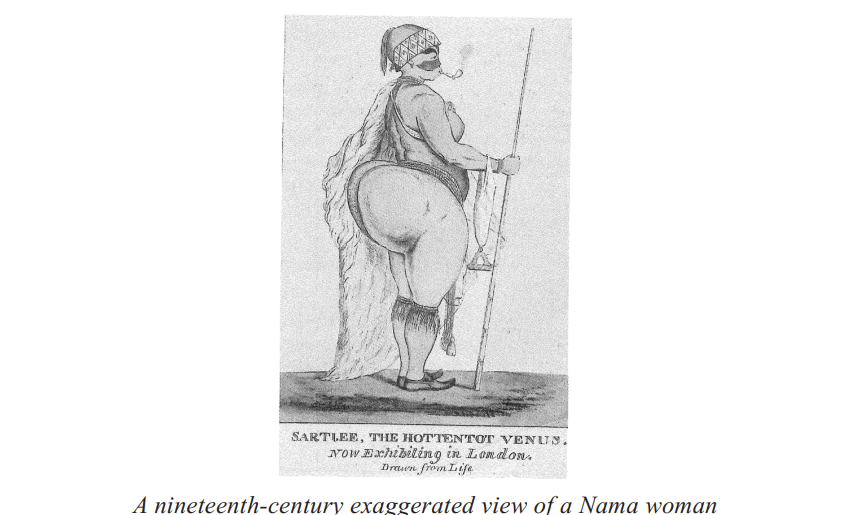
\includegraphics[width=0.75\linewidth]{image/Text5/Fig5.5.png}
\end{figure}

\noindent 38\\
Galton’s passion for quantification resulted in his developing many of the fundamental principles of modern statistics. It also yielded some clever observations. For example, he tested the efficacy of prayer. He figured that if prayer worked, those most prayed for should be at an advantage; to test the hypothesis he studied the longevity of British monarchs. Every Sunday, congregations in the Church of England following the Book of Common Prayer beseeched God to “Endue the king/queen plenteously with heavenly gifts; Grant him/her in health and wealth long to live.” Surely, Galton reasoned, the cumulative effect of all those prayers should be beneficial. In fact, prayer seemed ineffectual: he found that on average the monarchs died somewhat younger than other members of the British aristocracy.\\
高尔顿对量化的热衷促使他提出了现代统计学的许多基本原理。这也让他有了一些巧妙的观察。例如,他测试了祈祷的效果。他认为,如果祈祷有效,那些被人们最多地为之祈祷的人应该处于有利地位;为了验证这一假设,他研究了英国君主的寿命。每个星期天,英国国教的会众依照《公祷书》祈求上帝 “慷慨地赐予国王/女王属天的恩赐;赐予他/她健康和财富,使其长寿”。高尔顿推断,所有这些祈祷的累积效果肯定是有益的。事实上,祈祷似乎没有效果:他发现,平均而言,君主的寿命比英国贵族的其他成员要短一些 。\\

\noindent 39\\
Because of the Darwin connection—their common grandfather, Erasmus Darwin, too was one of the intellectual giants of his day—Galton was especially sensitive to the way in which certain lineages seemed to spawn disproportionately large numbers of prominent and successful people. In 1869 he published what would become the underpinning of all his ideas on eugenics, a treatise called *Hereditary Genius: An Inquiry into Its Laws and Consequences*. In it he purported to show that talent, like simple genetic traits such as the Hapsburg Lip, does indeed run in families; he recounted, for example, how some families had produced generation after generation of judges. His analysis largely neglected to take into account the effect of the environment: the son of a prominent judge is, after all, rather more likely to become a judge—by virtue of his father’s connections, if nothing else—than the son of a peasant farmer. Galton did not, however, completely overlook the effect of the environment, and it was he who first referred to the “nature/nurture” dichotomy, possibly in reference to Shakespeare’s irredeemable villain, Caliban, “a devil, a born devil, on whose nature/Nurture can never stick.”\\
由于与达尔文家族的关联——他们共同的祖父伊拉斯谟·达尔文也是他那个时代的知识巨匠之一——高尔顿对某些家族谱系中似乎不成比例地涌现出大量杰出成功人士的现象格外敏感。1869 年,他出版了一部论著《遗传的天才:对其规律和后果的探究》,这部著作成为了他所有优生学思想的基石。在书中,他试图证明,天赋如同哈布斯堡唇(一种简单的遗传特征)一样,确实在家族中代代相传;例如,他讲述了一些家族是如何一代又一代地出法官的。他的分析在很大程度上忽视了环境的影响:毕竟,一位杰出法官的儿子,即便没有其他因素,仅凭借父亲的人脉关系,也比农民的儿子更有可能成为法官。然而,高尔顿并没有完全忽视环境的影响,而且是他首次提出了 “先天/后天” 二分法,这可能是引用了莎士比亚笔下不可救药的反派角色凯列班的形象,“一个恶魔,天生的恶魔,后天教养对其本性毫无作用” 。\\

\noindent 40

\addtolength{\leftskip}{1cm}

\noindent The results of his analysis, however, left no doubt in Galton’s mind. \\
然而,他的分析结果让高尔顿坚信不疑。\\

\noindent I have no patience with the hypothesis occasionally expressed, and often implied, especially in tales written to teach children to be good, that babies are born pretty much alike, and that the sole agencies in creating differences between boy and boy, and man and man, are steady application and moral effort. It is in the most unqualified manner that I object to pretensions of natural equality.\\
我无法忍受那种偶尔被提及,且经常被暗示的假设,尤其是在教导孩子向善的故事中所表达的——婴儿出生时基本相似,而造成男孩与男孩之间、男人与男人之间差异的唯一因素,是坚持不懈的努力和道德上的修为。我毫无保留地反对这种关于天生平等的主张 。\\

\addtolength{\leftskip}{-1cm}

\noindent 41\\
A corollary of his conviction that these traits are genetically determined, he argued, was that it would be possible to “improve” the human stock by preferentially breeding gifted individuals, and preventing the less gifted from reproducing.\\
他认为,基于其 “这些特质是由基因决定的” 这一信念,必然会得出这样的推论:通过优先让有天赋的个体繁衍后代,并阻止天赋较低的人繁衍,就有可能 “改良” 人类种群。\\

\addtolength{\leftskip}{1cm}

\noindent It is easy . . . to obtain by careful selection a permanent breed of dogs or horses gifted with peculiar powers of running, or of doing anything else, so it would be quite practicable to produce a highly-gifted race of men by judicious marriages during several consecutive generations.\\
通过精心筛选,很容易培育出具有特殊奔跑能力或其他特殊能力的纯种狗或马,因此,通过连续几代人的明智婚配来培育出一个天赋极高的人类种族,也是完全可行的。 \\

\addtolength{\leftskip}{-1cm}


\noindent 42\\
Galton introduced the terms eugenics (literally “good in birth”) to describe this application of the basic principle of agricultural breeding to humans. In time, eugenics came to refer to “self-directed human evolution”: by making conscious choices about who should have children, eugenicists believed that they could head off the “eugenic crisis” precipitated in the Victorian imagination by the high rates of reproduction of inferior stock coupled with the typically small families of the superior middle classes.\\
高尔顿引入了“优生学”(字面意思是“生来优良”)这个术语,来描述将农业育种的基本原理应用于人类的情况。随着时间的推移,优生学被用来指代“自主导向的人类进化”:优生学家认为,通过有意识地选择谁应该生育后代,他们能够避免在维多利亚时代人们的想象中出现的“优生危机”,这种危机是由劣质种群的高生育率,以及优越的中产阶级普遍的小家庭规模共同引发的。 \\

[...]

\begin{figure}
    \centering
    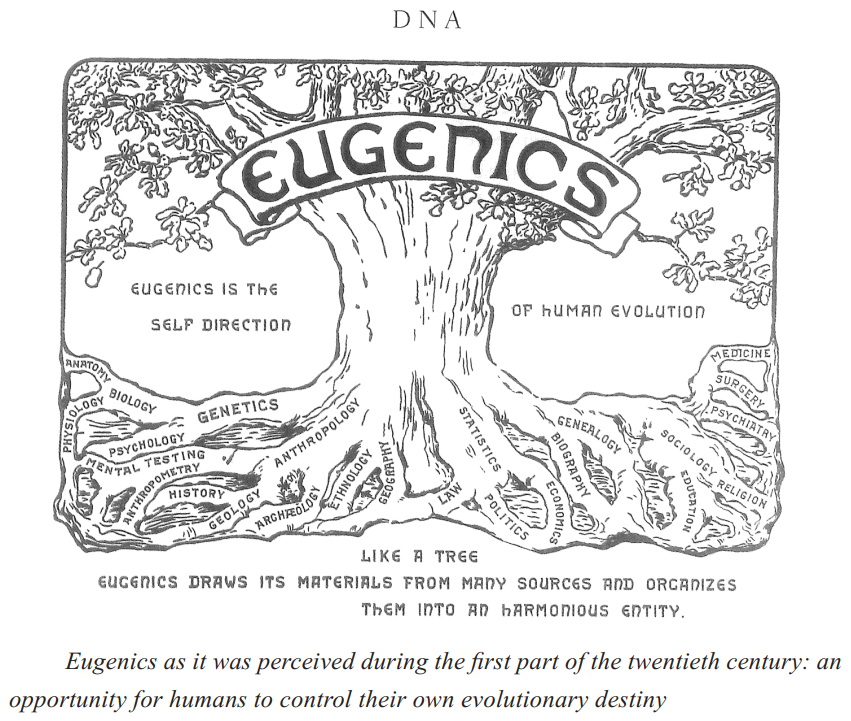
\includegraphics[width=0.75\linewidth]{image/Text5/Fig5.6.png}
\end{figure}

\begin{center}
CHAPTER TWO\\
THE DOUBLE HELIX: THIS IS LIFE\\
双螺旋结构:这就是生命 
\end{center}

\noindent 1\\
I got hooked on the gene during my third year at the University of Chicago. Until then, I had planned to be a naturalist and looked forward to a career far removed from the urban bustle of Chicago’s South Side, where I grew up. My change of heart was inspired not by an unforgettable teacher but a little book that appeared in 1944, *What Is Life?*, by the Austrian-born father of wave mechanics, Erwin Schrödinger. It grew out of several lectures he had given the year before at the Institute for Advanced Study in Dublin. That a great physicist had taken the time to write about biology caught my fancy. In those days, like most people, I considered chemistry and physics to be the “real” sciences, and theoretical physicists were science’s top dogs.\\
我在芝加哥大学读三年级时迷上了基因。在那之前,我原本计划成为一名博物学家,并且期待着从事一份远离我成长的芝加哥南区城市喧嚣的工作。让我改变想法的,不是一位令人难忘的老师,而是1944年出版的一本小书——《生命是什么?》,作者是出生于奥地利的波动力学之父埃尔温·薛定谔。这本书源于他前一年在都柏林高等研究院做的几场讲座。一位伟大的物理学家花时间撰写关于生物学的著作,这引起了我的兴趣。在那个时候,和大多数人一样,我认为化学和物理学才是“真正的”科学,而理论物理学家则是科学界的佼佼者。\\

\noindent 2\\
Schrödinger argued that life could be thought of in terms of storing and passing on biological information. Chromosomes were thus simply information bearers. Because so much information had to be packed into every cell, it must be compressed into what Schrödinger called a “hereditary code-script” embedded in the molecular fabric of chromosomes. To understand life, then, we would have to identify these molecules, and crack their code. He even speculated that understanding life—which would involve finding the gene—might take us beyond the laws of physics as we then understood them. Schrödinger’s book was tremendously influential. Many of those who would become major players in Act 1 of molecular biology’s great drama, including Francis Crick (a former physicist himself), had, like me, read *What Is Life?* and been impressed.\\
薛定谔认为,可以从储存和传递生物信息的角度来理解生命。因此,染色体仅仅是信息的载体。由于每个细胞都要承载大量的信息,这些信息必然被压缩成薛定谔所说的 “遗传密码本”,嵌入染色体的分子结构中。那么,要理解生命,我们就必须识别这些分子,并破解它们的密码。他甚至推测,理解生命——这其中包括找到基因——可能会让我们超越当时对物理定律的认知。薛定谔的这本书极具影响力。许多后来在分子生物学这一伟大篇章的第一幕中扮演重要角色的人,包括弗朗西斯·克里克(他本人曾是一名物理学家),都和我一样读过《生命是什么?》,并深受触动。 \\

\noindent 3\\
In my own case, Schrödinger struck a chord because I too was intrigued by the essence of life. A small minority of scientists still thought life depended upon a vital force emanating from an all - powerful god. But like most of my teachers, I disdained the very idea of vitalism. If such a “vital” force were calling the shots in nature’s game, there was little hope life would ever be understood through the methods of science. On the other hand, the notion that life might be perpetuated by means of an instruction book inscribed in a secret code appealed to me. What sort of molecular code could be so elaborate as to convey all the multitudinous wonder of the living world? And what sort of molecular trick could ensure that the code is exactly copied every time a chromosome duplicates?\\
就我个人而言,薛定谔的观点引起了我的共鸣,因为我也对生命的本质很感兴趣。一小部分科学家仍然认为生命依赖于一种来自全能上帝的生命力。但和我的大多数老师一样,我不屑于生机论这种观点。如果这种 “生命” 力量在主宰着自然界的一切,那么通过科学方法来理解生命就几乎没有希望。另一方面,生命可能通过一种用密码编写的 “说明书” 来延续的观点吸引了我。什么样的分子密码能够如此精妙,足以传达生物世界中所有纷繁复杂的奥秘呢?又是什么样的分子机制能够确保每次染色体复制时,密码都能被精确复制呢? \\

\noindent 4\\
At the time of Schrödinger’s Dublin lectures, most biologists supposed that proteins would eventually be identified as the primary bearers of genetic instruction. Proteins are molecular chains built up from twenty different building blocks, the amino acids. Because permutations in the order of amino acids along the chain are virtually infinite, proteins could, in principle, readily encode the information underpinning life’s extraordinary diversity. DNA then was not considered a serious candidate for the bearer of code-scripts, even though it was exclusively located on chromosomes and had been known about for some seventy-five years. In 1869, Friedrich Miescher, a Swiss biochemist working in Germany, had isolated from pus-soaked bandages supplied by a local hospital a substance he called “nuclein.” Because pus consists largely of white blood cells, which, unlike red blood cells, have nuclei and therefore DNA-containing chromosomes, Miescher had stumbled on a good source of DNA. When he later discovered that “nuclein” was to be found in chromosomes alone, Miescher understood that his discovery was indeed a big one. In 1893, he wrote: “Inheritance insures a continuity in form from generation to generation that lies even deeper than the chemical molecule. It lies in the structuring atomic groups. In this sense, I am a supporter of the chemical heredity theory.”\\
在薛定谔于都柏林举办讲座的时候,大多数生物学家认为,蛋白质最终会被确认为遗传指令的主要载体。蛋白质是由二十种不同的基本组成单位——氨基酸构成的分子链。由于氨基酸在链上的排列顺序几乎是无限的,从理论上来说,蛋白质可以轻松编码构成生命非凡多样性的信息。当时,DNA 并不被视为遗传密码本的有力候选者,尽管它仅存在于染色体上,且人们对它的认知已有七十五年左右。1869 年,在德国工作的瑞士生物化学家弗里德里希·米舍尔,从当地医院提供的沾满脓液的绷带中分离出一种他称之为 “核素” 的物质。因为脓液主要由白细胞组成,与红细胞不同,白细胞有细胞核,因此含有携带 DNA 的染色体,米舍尔偶然间找到了 DNA 的优质来源。后来,当他发现 “核素” 只存在于染色体中时,米舍尔意识到自己的发现意义重大。1893 年,他写道:“遗传确保了代与代之间形式上的连续性,这种连续性比化学分子层面更为深刻。它存在于原子团的结构之中。从这个意义上说,我支持化学遗传理论。” \\

\begin{figure}
    \centering
    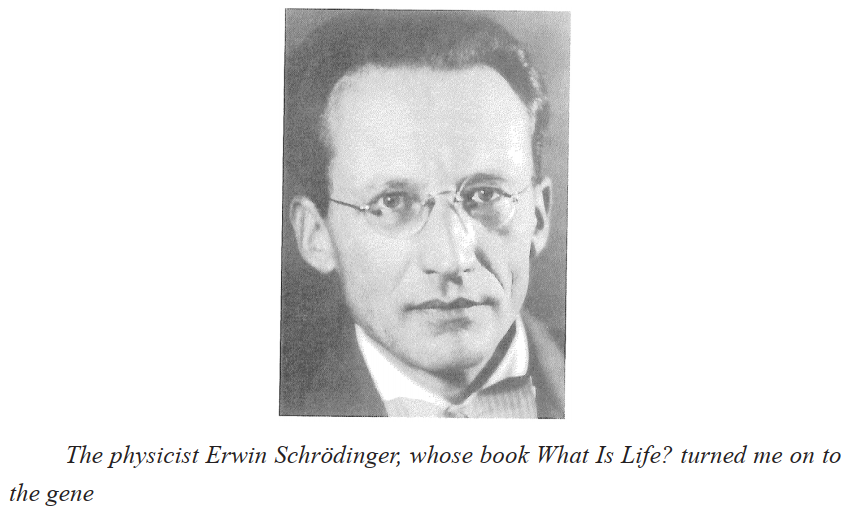
\includegraphics[width=0.75\linewidth]{image/Text5/Fig5.7.png}
\end{figure}

\noindent 5\\
Nevertheless, for decades afterward, chemistry would remain unequal to the task of analyzing the immense size and complexity of the DNA molecule. Only in the 1930s was DNA shown to be a long molecule containing four different chemical bases: adenine (A), guanine (G), thymine (T), and cytosine (C). But at the time of Schrödinger’s lectures, it was still unclear just how the subunits (called deoxynucleotides) of the molecule were chemically linked. Nor was it known whether DNA molecules might vary in their sequences of the four different bases. If DNA were indeed Schrödinger’s code-script, then the molecule would have to be capable of existing in an immense number of different forms. But back then it was still considered a possibility that one simple sequence like AGTC might be repeated over and over along the entire length of DNA chains.\\
然而,在那之后的几十年里,化学在分析 DNA 分子的巨大规模和复杂性方面仍力有不逮。直到20世纪30年代,人们才证明 DNA 是一种长分子,包含四种不同的化学碱基:腺嘌呤(A)、鸟嘌呤(G)、胸腺嘧啶(T)和胞嘧啶(C)。但在薛定谔举办讲座的时候,人们仍不清楚该分子的亚基(称为脱氧核苷酸)是如何通过化学键连接的。人们也不知道 DNA 分子中四种不同碱基的序列是否会有所不同。如果 DNA 确实是薛定谔所说的遗传密码本,那么这种分子必须能够以大量不同的形式存在。但在当时,人们仍认为像 AGTC 这样的简单序列有可能沿着 DNA 链不断重复 。 \\

\noindent 6\\
DNA did not move into the genetic limelight until 1944, when Oswald Avery’s lab at the Rockefeller Institute in New York City reported that the composition of the surface coats of pneumonia bacteria could be changed. This was not the result he and his junior colleagues, Colin MacLeod and Maclyn McCarty, expected.\\
直到1944年,DNA 才成为遗传学领域的焦点。当时,纽约洛克菲勒研究所奥斯瓦尔德·艾弗里的实验室报告称,肺炎细菌的表面荚膜成分可以改变。这并非是他和他的年轻同事科林·麦克劳德以及麦克林恩·麦卡蒂所预期的结果。\\

\noindent 7\\
For more than a decade Avery’s group had been following up on another most unexpected observation made in 1928 by Fred Griffith, a scientist in the British Ministry of Health. Griffith was interested in pneumonia and studied its bacterial agent, *Pneumococcus*. It was known that there were two strains, designated “smooth” (S) and “rough” (R) according to their appearance under the microscope. These strains differed not only visually but also in their virulence. Inject S bacteria into a mouse, and within a few days the mouse dies; inject R bacteria and the mouse remains healthy. It turns out that S bacterial cells have a coating that prevents the mouse’s immune system from recognizing the invader. The R cells have no such coating and are therefore readily attacked by the mouse’s immune defenses.\\
十多年来,艾弗里的研究小组一直在跟进英国卫生部科学家弗雷德·格里菲斯在1928年的一项极其意外的观察发现。格里菲斯对肺炎感兴趣,并研究了引发肺炎的细菌病原体——肺炎球菌。当时已知有两种菌株,根据它们在显微镜下的形态,分别被命名为 “光滑型”(S)和 “粗糙型”(R)。这些菌株不仅在外观上不同,而且在毒力上也有差异。将S型细菌注射到小鼠体内,几天内小鼠就会死亡;注射R型细菌,小鼠则保持健康。事实证明,S型细菌细胞有一层荚膜,可阻止小鼠的免疫系统识别入侵者。而R型细胞没有这种荚膜,因此很容易被小鼠的免疫防御系统攻击。 \\

\begin{figure}
    \centering
    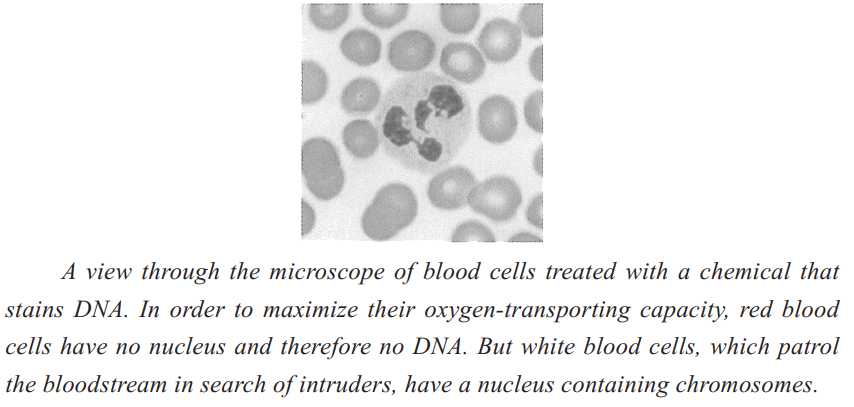
\includegraphics[width=0.75\linewidth]{image/Text5/Fig5.8.png}
\end{figure}

\noindent 8\\
Through his involvement with public health, Griffith knew that multiple strains had sometimes been isolated from a single patient, and so he was curious about how different strains might interact in his unfortunate mice. With one combination, he made a remarkable discovery: when he injected heat-killed S bacteria (harmless) and normal R bacteria (also harmless), the mouse died. How could two harmless forms of bacteria conspire to become lethal? The clue came when he isolated the *Pneumococcus* bacteria retrieved from the dead mice and discovered living S bacteria. It appeared the living innocuous R bacteria had acquired something from the dead S variant; whatever it was, that something had allowed the R in the presence of the heat-killed S bacteria to transform itself into a living killer S strain. Griffith confirmed that this change was for real by culturing the S bacteria from the dead mouse over several generations: the bacteria bred true for the S type, just as any regular S strain would. A genetic change had indeed occurred to the R bacteria injected into the mouse.\\
由于从事公共卫生工作,格里菲斯了解到有时能从单个患者体内分离出多种菌株,因此他很好奇不同的菌株在他用于实验的小鼠体内会如何相互作用。通过一种组合实验,他有了一个惊人的发现:当他将加热杀死的S型细菌(无害)和正常的R型细菌(也无害)注射到小鼠体内时,小鼠死亡了。两种无害的细菌怎么会共同作用而变得致命呢?当他从死亡小鼠体内分离出肺炎球菌,并发现了活的S型细菌时,线索出现了。看起来,活的、无害的R型细菌从死亡的S型细菌变体中获得了某种物质;不管这种物质是什么,它使得R型细菌在加热杀死的S型细菌存在的情况下,转化成了具有致死性的活S型菌株。格里菲斯通过对从死亡小鼠体内获取的S型细菌进行多代培养,证实了这种变化是真实的:这些细菌如同任何正常的S型菌株一样,能够稳定遗传S型的特性。注入小鼠体内的R型细菌确实发生了基因变化。 \\

\noindent 9\\
Though this transformation phenomenon seemed to defy all understanding, Griffith’s observations at first created little stir in the scientific world. This was partly because Griffith was intensely private and so averse to large gatherings that he seldom attended scientific conferences. Once, he had to be virtually forced to give a lecture. Bundled into a taxi and escorted to the hall by colleagues, he discoursed in a mumbled monotone, emphasizing an obscure corner of his microbiological work but making no mention of bacterial transformation. Luckily, however, not everyone overlooked Griffith’s breakthrough.\\
尽管这种转化现象似乎难以理解,但起初,格里菲斯的发现并没有在科学界引起多大轰动。部分原因是格里菲斯极为注重个人隐私,非常反感大型聚会,所以很少参加科学会议。有一次,他几乎是被强迫去做演讲。他被同事塞进出租车,护送到会场,讲话时含糊不清、语调单一,只强调了自己微生物研究中一个不为人知的方面,却对细菌转化只字未提。不过,幸运的是,并非所有人都忽视了格里菲斯的这一突破性发现。 \\

\noindent 10\\
Oswald Avery was also interested in the sugarlike coats of the *Pneumococcus*. He set out to duplicate Griffith’s experiment in order to isolate and characterize whatever it was that had caused those R cells to change to the S type. In 1944 Avery, MacLeod, and McCarty published their results: an exquisite set of experiments showing unequivocally that DNA was the transforming principle. Culturing the bacteria in the test tube rather than in mice made it much easier to search for the chemical identity of the transforming factor in the heat-killed S cells. Methodically destroying one by one the biochemical components of the heat-treated S cells, Avery and his group looked to see whether transformation was prevented. First they degraded the sugarlike coat of the S bacteria. Transformation still occurred: the coat was not the transforming principle. Next they used a mixture of two protein-destroying enzymes, trypsin and chymotrypsin, to degrade virtually all the proteins in the S cells. To their surprise, transformation was again unaffected. Next they tried an enzyme (RNase) that breaks down RNA (ribonucleic acid), a second class of nucleic acids similar to DNA and possibly involved in protein synthesis. Again transformation occurred. Finally, they came to DNA, exposing the S bacterial extracts to the DNA-destroying enzyme, DNase. This time they hit a home run. All S-inducing activity ceased completely. The transforming factor was DNA.\\
奥斯瓦尔德·艾弗里也对肺炎球菌的多糖荚膜感兴趣。他着手重复格里菲思的实验,试图分离并鉴定出使那些R型细胞转变为S型细胞的物质。1944年,艾弗里、麦克劳德和麦卡蒂发表了他们的实验结果:一系列精妙的实验明确表明,DNA就是转化因子。在试管中而非在小鼠体内培养细菌,使得寻找热灭活S型细菌中转化因子的化学本质变得容易得多。艾弗里及其团队有条不紊地逐一破坏热处理后的S型细胞的生化成分,观察转化是否会被阻止。首先,他们降解了S型细菌的多糖荚膜。但转化仍然发生了,这表明荚膜不是转化因子。接下来,他们使用了两种能分解蛋白质的酶(胰蛋白酶和糜蛋白酶)的混合物,几乎降解了S型细胞中的所有蛋白质。令他们惊讶的是,转化再次未受影响。然后,他们尝试使用一种能分解RNA(核糖核酸,一种与DNA类似且可能参与蛋白质合成的核酸)的酶(RNA酶),转化还是发生了。最后,他们研究到了DNA,将S型细菌提取物暴露于能分解DNA的酶(DNA酶)中。这次他们大获成功,所有诱导S型细菌产生的活性完全停止了。由此可知,转化因子就是DNA。\\ 

\noindent 11\\
In part because of its bombshell implications, the resulting February 1944 paper by Avery, MacLeod, and McCarty met with a mixed response. Many geneticists accepted their conclusions. After all, DNA was found on every chromosome; why shouldn’t it be the genetic material? By contrast, however, most biochemists expressed doubt that DNA was a complex enough molecule to act as the repository of such a vast quantity of biological information. They continued to believe that proteins, the other component of chromosomes, would prove to be the hereditary substance. In principle, as the biochemists rightly noted, it would be much easier to encode a vast body of complex information using the twenty - letter amino - acid alphabet of proteins than the four - letter nucleotide alphabet of DNA. Particularly vitriolic in his rejection of DNA as the genetic substance was Avery’s own colleague at the Rockefeller Institute, the protein chemist Alfred Mirsky. By then, however, Avery was no longer scientifically active. The Rockefeller Institute had mandatorily retired him at age sixty - five.\\
部分由于其惊人的意义,艾弗里、麦克劳德和麦卡蒂于1944年2月发表的论文引发了褒贬不一的反响。许多遗传学家接受了他们的结论。毕竟,每条染色体上都有DNA,它为什么不能是遗传物质呢?然而,相比之下,大多数生物化学家对此表示怀疑,他们认为DNA分子的复杂程度不足以成为如此大量生物信息的储存库。他们仍然坚信,染色体的另一种组成成分——蛋白质,才会被证明是遗传物质。从理论上讲,正如生物化学家们正确指出的,用由20种氨基酸组成的 “字母表” 来编码大量复杂信息,要比用由4种核苷酸组成的DNA “字母表” 容易得多。艾弗里在洛克菲勒研究所的同事、蛋白质化学家阿尔弗雷德·米尔施基,对DNA作为遗传物质的观点尤为反感。然而,那时艾弗里已经不再活跃于科研领域,洛克菲勒研究所在他65岁时强制他退休了。\\

\noindent 12\\
Avery missed out on more than the opportunity to defend his work against the attacks of his colleagues: He was never awarded the Nobel Prize, which was certainly his due, for identifying DNA as the transforming principle. Because the Nobel committee makes its records public fifty years following each award, we now know that Avery’s candidacy was blocked by the Swedish physical chemist Einar Hammarsten. Though Hammarsten’s reputation was based largely on his having produced DNA samples of unprecedented high quality, he still believed genes to be an undiscovered class of proteins. In fact, even after the double helix was found, Hammarsten continued to insist that Avery should not receive the prize until after the mechanism of DNA transformation had been completely worked out. Avery died in 1955; had he lived only a few more years, he would almost certainly have gotten the prize.\\
艾弗里错过的不仅仅是为自己的研究成果抵御同事抨击的机会:他因确定DNA是(细菌)转化要素,本应获得诺贝尔奖,却从未获此殊荣。由于诺贝尔奖委员会在每次颁奖五十年后会公布相关记录,我们现在得知,艾弗里的候选人资格被瑞典物理化学家埃纳尔·哈马斯坦否决了。尽管哈马斯坦的声誉主要源于他制备出了前所未有的高质量DNA样本,但他仍然认为基因是一类尚未被发现的蛋白质。事实上,即使在DNA双螺旋结构被发现之后,哈马斯坦仍坚持认为,在DNA转化机制被完全阐明之前,艾弗里不应获奖。艾弗里于1955年去世;要是他能再多活几年,几乎肯定会获得诺贝尔奖。\\

\noindent 13\\
When I arrived at Indiana University in the fall of 1947 with plans to pursue the gene for my Ph.D. thesis, Avery’s paper came up over and over in conversations.
By then, no one doubted the reproducibility of his results, and more recent work coming out of the Rockefeller Institute made it all the less likely that proteins would prove to be the genetic actors in bacterial transformation. DNA had at last become an important objective for chemists setting their sights on the next breakthrough. In Cambridge, England, the canny Scottish chemist Alexander Todd rose to the challenge of identifying the chemical bonds that linked together nucleotides in DNA. By early 1951, his lab had proved that these links were always the same, such that the backbone of the DNA molecule was very regular. During the same period, the Austrian-born refugee Erwin Chargaff, at the College of Physicians and Surgeons of Columbia University, used the new technique of paper chromatography to measure the relative amounts of the four DNA bases in DNA samples extracted from a variety of vertebrates and bacteria. While some species had DNA in which adenine and thymine predominated, others had DNA with more guanine and cytosine. The possibility thus presented itself that no two DNA molecules had the same composition.\\
1947年秋天,我来到印第安纳大学,打算以基因作为博士论文的研究方向,艾弗里的论文在各种讨论中反复被提及。
那时,没人怀疑他的实验结果具有可重复性,而且洛克菲勒研究所最新的研究成果,使蛋白质更不可能被证明是细菌转化中的遗传物质。对于期望取得下一个重大突破的化学家们来说,DNA 最终成为了一个重要的研究目标。在英国剑桥,精明的苏格兰化学家亚历山大·托德接受了挑战,去确定 DNA 中连接核苷酸的化学键。到1951年初,他的实验室已证明这些连接总是相同的,这使得 DNA 分子的骨架非常规则。同一时期,出生于奥地利的难民埃尔文·查格夫,在哥伦比亚大学的内科与外科医师学院,运用纸色谱分析法这一新技术,测量了从多种脊椎动物和细菌中提取的 DNA 样本里四种 DNA 碱基的相对含量。有些物种的 DNA 中腺嘌呤和胸腺嘧啶占主导,而另一些物种的 DNA 中鸟嘌呤和胞嘧啶含量更高。由此可见,没有两个 DNA 分子的组成是相同的,这种可能性是存在的。 \\

\noindent 14\\
At Indiana I joined a small group of visionary scientists, mostly physicists and chemists, studying the reproductive process of the viruses that attack bacteria (bacteriophages—“phages” for short). The Phage Group was born when my Ph.D. supervisor, the Italian-trained medic Salvador Luria and his close friend, the German-born theoretical physicist Max Delbrück, teamed up with the American physical chemist Alfred Hershey. During World War II both Luria and Delbrück were considered enemy aliens, and thus ineligible to serve in the war effort of American science, even though Luria, a Jew, had been forced to leave France for New York City and Delbrück had fled Germany as an objector to Nazism. Thus excluded, they continued to work in their respective university labs—Luria at Indiana and Delbrück at Vanderbilt—and collaborated on phage experiments during successive summers at Cold Spring Harbor. In 1943, they joined forces with the brilliant but taciturn Hershey, then doing phage research of his own at Washington University in St. Louis.\\
在印第安纳大学,我加入了一个由有远见卓识的科学家组成的小团队,成员大多是物理学家和化学家,他们正在研究攻击细菌的病毒(噬菌体,简称 “phages”)的繁殖过程。噬菌体研究小组的成立,源于我的博士导师、在意大利接受医学教育的萨尔瓦多·卢里亚,以及他的挚友、出生于德国的理论物理学家马克斯·德尔布吕克,与美国物理化学家阿尔弗雷德·赫尔希的合作。第二次世界大战期间,卢里亚和德尔布吕克都被视为敌国侨民,因此没有资格参与美国科学界的战时工作,尽管身为犹太人的卢里亚被迫从法国前往纽约,而德尔布吕克作为纳粹主义的反对者逃离了德国。尽管被排除在外,他们仍在各自的大学实验室继续工作——卢里亚在印第安纳大学,德尔布吕克在范德堡大学——并在接下来的几个夏天于冷泉港合作进行噬菌体实验。1943 年,他们与才华横溢但沉默寡言的赫尔希携手合作,当时赫尔希正在圣路易斯的华盛顿大学开展自己的噬菌体研究。 \\

\noindent 15\\
The Phage Group’s program was based on its belief that phages, like all viruses, were in effect naked genes. This concept had first been proposed in 1922 by the imaginative American geneticist Herman J. Muller, who three years later demonstrated that X rays cause mutations. His belated Nobel Prize came in 1946, just after he joined the faculty of Indiana University. It was his presence, in fact, that led me to Indiana. Having started his career under T.H. Morgan, Muller knew better than anyone else how genetics had evolved during the first half of the twentieth century, and I was enthralled by his lectures during my first term. His work on fruit flies (*Drosophila*), however, seemed to me to belong more to the past than to the future, and I only briefly considered doing thesis research under his supervision. I opted instead for Luria’s phages, an even speedier experimental subject than *Drosophila*: genetic crosses of phages done one day could be analyzed the next.\\
噬菌体研究小组的研究计划基于这样一种信念:噬菌体和所有病毒一样,实际上都是裸露的基因。这一概念最早由富有想象力的美国遗传学家赫尔曼·J·穆勒在1922 年提出,三年后,他证明了 X 射线会引发突变。1946 年,在他加入印第安纳大学任教后不久,他终于获得了诺贝尔奖。事实上,正是因为他在那里,我才选择了印第安纳大学。穆勒在托马斯·亨特·摩根手下开始了他的职业生涯,他比任何人都更清楚20世纪上半叶遗传学的发展历程,我在第一学期就被他的讲座深深吸引。然而,在我看来,他关于果蝇(黑腹果蝇)的研究更像是属于过去,而非未来,我只是短暂考虑过在他的指导下进行论文研究。相反,我选择了卢里亚的噬菌体研究,噬菌体是比果蝇更快的实验对象:今天进行的噬菌体杂交实验,明天就可以进行分析。\\

\noindent 16\\
For my Ph.D. thesis research, Luria had me follow in his footsteps by studying how X rays killed phage particles. Initially I had hoped to show that viral death was caused by damage to phage DNA. Reluctantly, however, I eventually had to concede that my experimental approach could never give unambiguous answers at the chemical level. I could draw only biological conclusions. Even though phages were indeed effectively naked genes, I realized that the deep answers the Phage Group was seeking could be arrived at only through advanced chemistry. DNA somehow had to transcend its status as an acronym; it had to be understood as a molecular structure in all its chemical detail.\\
在我的博士论文研究中,卢里亚让我追随他的脚步,研究X射线是如何杀死噬菌体颗粒的。起初,我希望证明病毒的死亡是由噬菌体DNA受损导致的。然而,我最终不得不无奈地承认,我的实验方法永远无法在化学层面给出明确的答案,我只能得出生物学层面的结论。尽管噬菌体实际上确实是裸露的基因,但我意识到,噬菌体研究小组所追寻的深层次答案,只有通过高深的化学知识才能找到。DNA不能仅仅停留在一个缩写词的层面;我们必须从分子结构的所有化学细节上去理解它。\\

\noindent 17\\
Upon finishing my thesis, I saw no alternative but to move to a lab where I could study DNA chemistry. Unfortunately, however, knowing almost no pure chemistry, I would have been out of my depth in any lab attempting difficult experiments in organic or physical chemistry. I therefore took a postdoctoral fellowship in the Copenhagen lab of the biochemist Herman Kalckar in the fall of 1950. He was studying the synthesis of the small molecules that make up DNA, but I figured out quickly that his biochemical approach would never lead to an understanding of the essence of the gene. Every day spent in his lab would be one more day’s delay in learning how DNA carried genetic information.\\
完成博士论文后,我别无选择,只能前往一个能让我研究DNA化学的实验室。然而不幸的是,由于我几乎不懂纯化学知识,在任何试图开展有机化学或物理化学复杂实验的实验室里,我都会力不从心。因此,1950年秋天,我在生物化学家赫尔曼·卡尔卡的哥本哈根实验室获得了一个博士后职位。他当时正在研究构成DNA的小分子的合成,但我很快意识到,他的生物化学研究方法永远无法让我们理解基因的本质。在他的实验室里待的每一天,都会让我在了解DNA如何携带遗传信息这件事上多耽搁一天。\\

\noindent 18\\
My Copenhagen year nonetheless ended productively. To escape the cold Danish spring, I went to the Zoological Station at Naples during April and May. During my last week there, I attended a small conference on X-ray diffraction methods for determining the 3-D structure of molecules. X-ray diffraction is a way of studying the atomic structure of any molecule that can be crystallized. The crystal is bombarded with X rays, which bounce off its atoms and are scattered. The scatter pattern gives information about the structure of the molecule but, taken alone, is not enough to solve the structure. The additional information needed is the “phase assignment,” which deals with the wave properties of the molecule. Solving the phase problem was not easy, and at that time only the most audacious scientists were willing to take it on. Most of the successes of the diffraction method had been achieved with relatively simple molecules.\\
尽管如此,我在哥本哈根的这一年还是颇有收获地结束了。为了躲避丹麦寒冷的春天,我在4月和5月前往那不勒斯的动物研究所。在那里的最后一周,我参加了一个关于利用X射线衍射法测定分子三维结构的小型会议。X射线衍射是一种研究任何可结晶分子原子结构的方法。用X射线轰击晶体,X射线会从晶体的原子上反弹并发生散射。散射图样能提供有关分子结构的信息,但仅靠它不足以确定分子结构。还需要额外的信息,即 “相位确定”,这涉及分子的波动特性。解决相位问题并不容易,当时只有最无畏的科学家才愿意尝试。衍射方法的大多数成功案例都来自相对简单的分子。\\

\noindent 19\\
My expectations for the conference were low. I believed that a three-dimensional understanding of protein structure, or for that matter of DNA, was more than a decade away. Disappointing earlier X-ray photos suggested that DNA was particularly unlikely to yield up its secrets via the X-ray approach. These results were not surprising since the exact sequences of DNA were expected to differ from one individual molecule to another. The resulting irregularity of surface configurations would understandably prevent the long thin DNA chains from lying neatly side by side in the regular repeating patterns required for X-ray analysis to be successful.\\
我对这次会议期望不高。我认为,要从三维层面理解蛋白质结构,或者就此而言理解DNA结构,至少还得等上十多年。早期令人失望的X射线照片表明,DNA尤其不太可能通过X射线分析的方法揭示其奥秘。这些结果并不令人意外,因为不同的DNA分子,其确切序列预计都是不同的。由此产生的表面形态的不规则性,会阻碍细长的DNA链整齐地并排排列成X射线分析所需的规则重复模式,这是可以理解的。\\

\noindent 20\\
It was therefore a surprise and a delight to hear the last-minute talk on DNA by a thirty-four-year-old Englishman named Maurice Wilkins from the Biophysics Lab of King’s College, London. Wilkins was a physicist who during the war had worked on the Manhattan Project. For him, as for many of the other scientists involved, the actual deployment of the bomb on Hiroshima and Nagasaki, supposedly the culmination of all their work, was profoundly disillusioning.\\
因此,当听到来自伦敦国王学院生物物理实验室、34岁的英国科学家莫里斯·威尔金斯在最后一刻做的关于DNA的报告时,我既惊讶又欣喜。威尔金斯是一名物理学家,战时曾参与曼哈顿计划。对他以及许多其他参与该计划的科学家来说,原子弹实际被投放在广岛和长崎,这本应是他们所有工作的顶峰,却让他们深感失望。\\

\begin{figure}
    \centering
    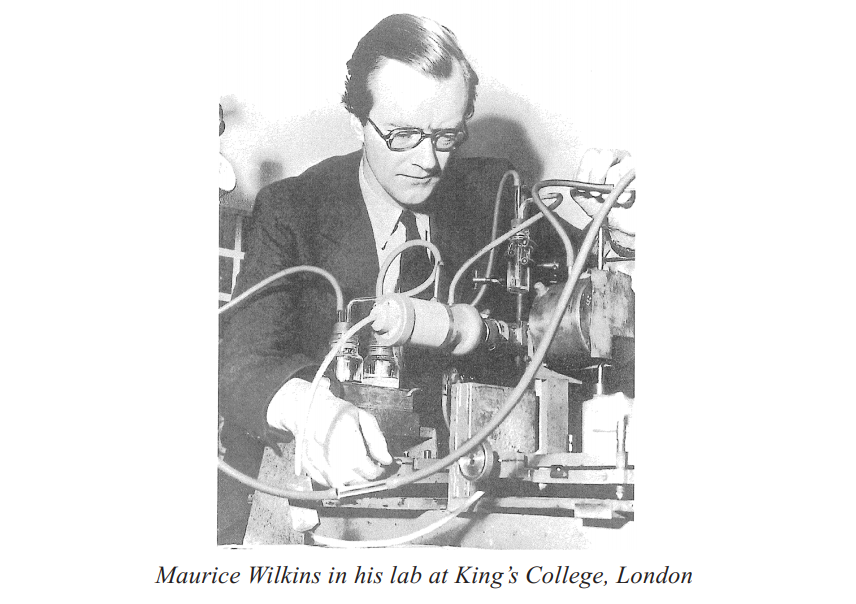
\includegraphics[width=0.75\linewidth]{image/Text5/Fig5.9.png}
\end{figure}

\noindent 21\\
He considered forsaking science altogether to become a painter in Paris, but biology intervened. He too had read Schrödinger’s book, and was now tackling DNA with X-ray diffraction.\\
他曾考虑彻底放弃科学,去巴黎当一名画家,但生物学改变了他的想法。他也读过薛定谔的书,如今正用X射线衍射法研究DNA。\\

\noindent 22\\
He displayed a photograph of an X-ray diffraction pattern he had recently obtained, and its many precise reflections indicated a highly regular crystalline packing. DNA, one had to conclude, must have a regular structure, the elucidation of which might well reveal the nature of the gene. Instantly I saw myself moving to London to help Wilkins find the structure. My attempts to converse with him after his talk, however, went nowhere. All I got for my efforts was a declaration of his conviction that much hard work lay ahead.\\
他展示了一张近期获得的X射线衍射图谱照片,图谱上众多精确的反射图案表明存在高度规则的晶体堆积。由此可以得出结论,DNA必定具有规则的结构,对其结构的阐释很可能会揭示基因的本质。我当即就想着要去伦敦,帮助威尔金斯探寻DNA的结构。然而,他演讲结束后,我试图与他交流,却一无所获。我得到的回应,仅仅是他坚信前路仍有大量艰苦的工作要做。\\

\noindent 23\\
While I was hitting consecutive dead ends, back in America the world’s preeminent chemist, Caltech’s Linus Pauling, announced a major triumph: he had found the exact arrangement in which chains of amino acids (called polypeptides) fold up in proteins, and called his structure the α-helix (alpha helix). That it was Pauling who made this breakthrough was no surprise: he was a scientific superstar. His book *The Nature of the Chemical Bond* essentially laid the foundation of modern chemistry, and, for chemists of the day, it was the Bible. Pauling had been a precocious child. When he was nine, his father, a druggist in Oregon, wrote to the *Oregonian* newspaper requesting suggestions of reading matter for his bookish son, adding that he had already read the Bible and Darwin’s *Origin of Species*. But the early death of Pauling’s father, which brought the family to financial ruin, makes it remarkable that the promising young man managed to get an education at all.\\
在我屡屡碰壁之时,远在美国的世界顶尖化学家、加州理工学院的莱纳斯·鲍林宣布了一项重大成果:他发现了氨基酸链(称为多肽)在蛋白质中折叠的精确方式,并将这种结构称为α-螺旋(阿尔法螺旋)。取得这一突破的是鲍林,这并不令人意外,因为他是科学界的超级巨星。他的著作《化学键的本质》从根本上奠定了现代化学的基础,对于当时的化学家而言,这本书就是 “圣经”。鲍林自幼聪慧过人。九岁时,他在俄勒冈州当药剂师的父亲给《俄勒冈人报》写信,希望为他爱读书的儿子推荐一些读物,还提到他儿子已经读过《圣经》和达尔文的《物种起源》。然而,鲍林父亲的早逝让家庭陷入经济困境,在这种情况下,这位前途无量的年轻人还能接受教育,实在难能可贵。\\

\noindent 24\\
As soon as I returned to Copenhagen I read about Pauling’s α-helix. To my surprise, his model was not based on a deductive leap from experimental X-ray diffraction data. Instead, it was Pauling’s long experience as a structural chemist that had emboldened him to infer which type of helical fold would be most compatible with the underlying chemical features of the polypeptide chain. Pauling made scale models of the different parts of the protein molecule, working out plausible schemes in three dimensions. He had reduced the problem to a kind of three-dimensional jigsaw puzzle in a way that was simple yet brilliant.\\
我一回到哥本哈根,就了解了鲍林的α-螺旋理论。令我惊讶的是,他的模型并非基于从X射线衍射实验数据中得出的推导结论。相反,正是鲍林作为结构化学家的长期经验,让他有底气推断出哪种螺旋折叠方式与多肽链的基本化学特征最为契合。鲍林制作了蛋白质分子不同部分的比例模型,构建出了合理的三维结构方案。他把这个问题简化成了一种三维拼图游戏,方法简单却又十分巧妙。\\

\noindent 25\\
Whether the α-helix was correct—in addition to being pretty—was now the question. Only a week later, I got the answer. Sir Lawrence Bragg, the English inventor of X-ray crystallography and 1915 Nobel laureate in Physics, came to Copenhagen and excitedly reported that his junior colleague, the Austrian-born chemist Max Perutz, had ingeniously used synthetic polypeptides to confirm the correctness of Pauling’s α-helix. It was a bittersweet triumph for Bragg’s Cavendish Laboratory. The year before, they had completely missed the boat in their paper outlining possible helical folds for polypeptide chains.\\
如今的问题是,α-螺旋结构除了看起来精巧之外,是否正确。仅仅一周后,我就得到了答案。英国X射线晶体学的发明者、1915 年诺贝尔物理学奖得主劳伦斯·布拉格爵士来到哥本哈根,兴奋地报告说,他的年轻同事、出生于奥地利的化学家马克斯·佩鲁茨巧妙地利用合成多肽证实了鲍林的α-螺旋结构是正确的。对于布拉格所在的卡文迪许实验室而言,这是一场喜忧参半的胜利。前一年,他们在概述多肽链可能的螺旋折叠方式的论文中完全错失了机会。\\

\begin{figure}
    \centering
    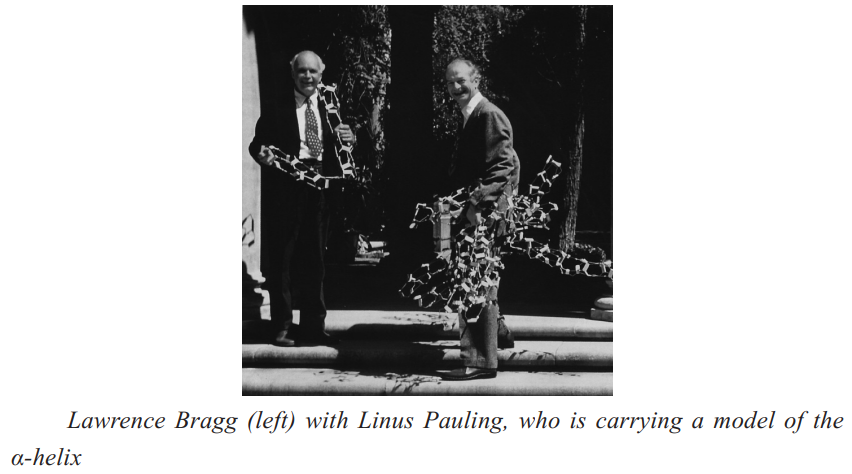
\includegraphics[width=0.75\linewidth]{image/Text5/Fig5.10.png}
\end{figure}

\noindent 26\\
By then Salvador Luria had tentatively arranged for me to take up a research position at the Cavendish. Located at Cambridge University, this was the most famous laboratory in all of science. Here Ernest Rutherford first described the structure of the atom. Now it was Bragg’s own domain, and I was to work as apprentice to the English chemist John Kendrew, who was interested in determining the 3-D structure of the protein myoglobin. Luria advised me to visit the Cavendish as soon as possible. With Kendrew in the States, Max Perutz would check me out. Together, Kendrew and Perutz had earlier established the Medical Research Council (MRC) Unit for the Study of the Structure of Biological Systems.\\
那时,萨尔瓦多·卢里亚已经初步为我安排了在卡文迪许实验室的一个研究职位。该实验室位于剑桥大学,是科学界最负盛名的实验室。欧内斯特·卢瑟福就是在这里首次描述了原子结构。如今这里是布拉格的 “领地”,我将作为英国化学家约翰·肯德鲁的助手开展工作,他致力于确定肌红蛋白的三维结构。卢里亚建议我尽快去卡文迪许实验室看看。由于肯德鲁当时在美国,马克斯·佩鲁茨会对我进行考察。此前,肯德鲁和佩鲁茨共同创立了医学研究委员会(MRC)生物系统结构研究小组。\\

\noindent 27\\
A month later in Cambridge, Perutz assured me that I could quickly master the necessary X-ray diffraction theory and should have no difficulty fitting in with the others in their tiny MRC Unit. To my relief, he was not put off by my biology background. Nor was Lawrence Bragg, who briefly came down from his office to look me over.\\
一个月后,在剑桥,佩鲁茨向我保证,我能很快掌握必要的X射线衍射理论,并且在医学研究委员会这个小研究小组里,与其他人相处也不会有什么困难。令我宽慰的是,他没有因为我的生物学背景而对我有偏见。劳伦斯·布拉格也是如此,他短暂地从办公室下来,对我进行了一番打量。\\

\noindent 28\\
I was twenty-three when I arrived back at the MRC Unit in Cambridge in early October. I found myself sharing space in the biochemistry room with a thirty-five-year-old ex-physicist, Francis Crick, who had spent the war working on magnetic mines for the Admiralty. When the war ended, Crick had planned to stay on in military research, but, on reading Schrödinger’s *What Is Life?*, he had moved toward biology. Now he was at the Cavendish to pursue the 3-D structure of proteins for his Ph.D.\\
10月初,我回到剑桥的医学研究委员会研究小组,那时我23岁。我和一位35岁的前物理学家弗朗西斯·克里克共用生物化学实验室的空间,他在战时曾为英国海军部研究磁性水雷。战争结束后,克里克原本打算继续从事军事研究,但读了薛定谔的《生命是什么?》之后,他转向了生物学领域。如今,他在卡文迪许实验室攻读博士学位,研究蛋白质的三维结构。\\

\noindent 29\\
Crick was always fascinated by the intricacies of important problems. His endless questions as a child compelled his weary parents to buy him a children’s encyclopedia, hoping that it would satisfy his curiosity. But it only made him insecure: he confided to his mother his fear that everything would have been discovered by the time he grew up, leaving him nothing to do. His mother reassured him (correctly, as it happened) that there would still be a thing or two for him to figure out.\\
克里克总是痴迷于重要问题的复杂之处。小时候,他接连不断的提问让疲惫的父母不得不给他买了一本儿童百科全书,希望能满足他的好奇心。但这反而让他感到不安,他向母亲吐露,担心等自己长大后,所有的东西都已被发现,那样他就无事可做了。他母亲安慰他(事实证明这是对的),说总会有一两件事等着他去探索发现。\\

\noindent 30\\
A great talker, Crick was invariably the center of attention in any gathering. His booming laugh was forever echoing down the hallways of the Cavendish. As the MRC Unit’s resident theoretician, he used to come up with a novel insight at least once a month, and he would explain his latest idea at great length to anyone willing to listen. The morning we met he lit up when he learned that my objective in coming to Cambridge was to learn enough crystallography to have a go at the DNA structure. Soon I was asking Crick’s opinion about using Pauling’s model-building approach to go directly for the structure. Would we need many more years of diffraction experimentation before modeling would be practicable? To bring us up to speed on the status of DNA structural studies, Crick invited Maurice Wilkins, a friend since the end of the war, up from London for Sunday lunch. Then we could learn what progress Wilkins had made since his talk in Naples.\\
克里克很健谈,在任何聚会中他总是众人关注的焦点。他爽朗的笑声常常在卡文迪许实验室的走廊里回荡。作为医学研究委员会研究小组的常驻理论家,他过去每个月至少会提出一个新颖的见解,而且会向任何愿意倾听的人详尽地解释他的最新想法。我们见面的那天早上,当他得知我来剑桥的目标是学习足够的晶体学知识,以便研究DNA结构时,他一下子来了兴致。很快,我就向克里克请教关于采用鲍林的模型构建方法直接研究DNA结构的看法。在能够实际构建模型之前,我们还需要进行很多年的衍射实验吗?为了让我们了解DNA结构研究的最新进展,克里克邀请了自二战结束后就相识的朋友莫里斯·威尔金斯从伦敦过来吃周日午餐。这样我们就能知道威尔金斯自从在那不勒斯做报告之后取得了哪些进展。\\

\begin{figure}
    \centering
    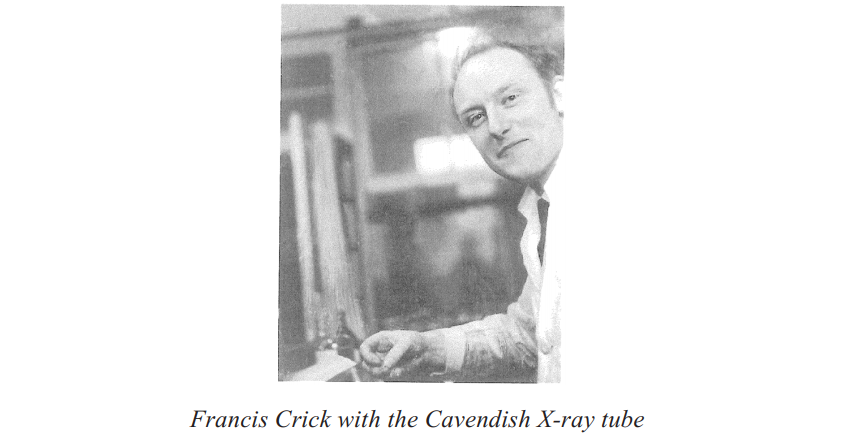
\includegraphics[width=0.75\linewidth]{image/Text5/Fig5.11.png}
\end{figure}

\noindent 31\\
Wilkins expressed his belief that DNA’s structure was a helix, formed by several chains of linked nucleotides twisted around each other. All that remained to be settled was the number of chains. At the time, Wilkins favored three on the basis of his density measurements of DNA fibers. He was keen to start model-building, but he had run into a roadblock in the form of a new addition to the King’s College Biophysics Unit, Rosalind Franklin.\\
威尔金斯表示,他认为DNA的结构是螺旋形,由几条相互缠绕的核苷酸链组成。剩下有待确定的就是链的数量。当时,基于对DNA纤维的密度测量,威尔金斯倾向于三条链的说法。他迫切地想要开始搭建模型,但却遇到了一个阻碍——伦敦国王学院生物物理小组新加入的成员罗莎琳德·富兰克林。\\

\noindent 32\\
A thirty-one-year-old Cambridge-trained physical chemist, Franklin was an obsessively professional scientist; for her twenty-ninth birthday all she requested was her own subscription to her field’s technical journal, *Acta Crystallographica*. Logical and precise, she was impatient with those who acted otherwise. And she was given to strong opinions, once describing her Ph.D. thesis adviser, Ronald Norrish, a future Nobel Laureate, as “stupid, bigoted, deceitful, ill-mannered and tyrannical.” Outside the laboratory, she was a determined and gutsy mountaineer, and, coming from the upper echelons of London society, she belonged to a more rarefied social world than most scientists. At the end of a hard day at the bench, she would occasionally change out of her lab coat into an elegant evening gown and disappear into the night.\\
富兰克林31岁,是一位毕业于剑桥大学的物理化学家,她对科研工作极为执着。29岁生日时,她唯一想要的就是订阅自己所在领域的学术期刊《晶体学报》。她思维逻辑严谨、精确,对行事风格不同的人缺乏耐心。她观点鲜明,曾将自己的博士论文导师、日后的诺贝尔奖得主罗纳德·诺里什描述为 “愚蠢、偏执、虚伪、举止粗俗且专横”。在实验室之外,她是个意志坚定、勇敢无畏的登山爱好者。她出身于伦敦上流社会,所处的社交圈子比大多数科学家更为高雅。在实验室辛苦工作一天后,她偶尔会脱下实验服,换上优雅的晚礼服,消失在夜色中。\\

\begin{figure}
    \centering
    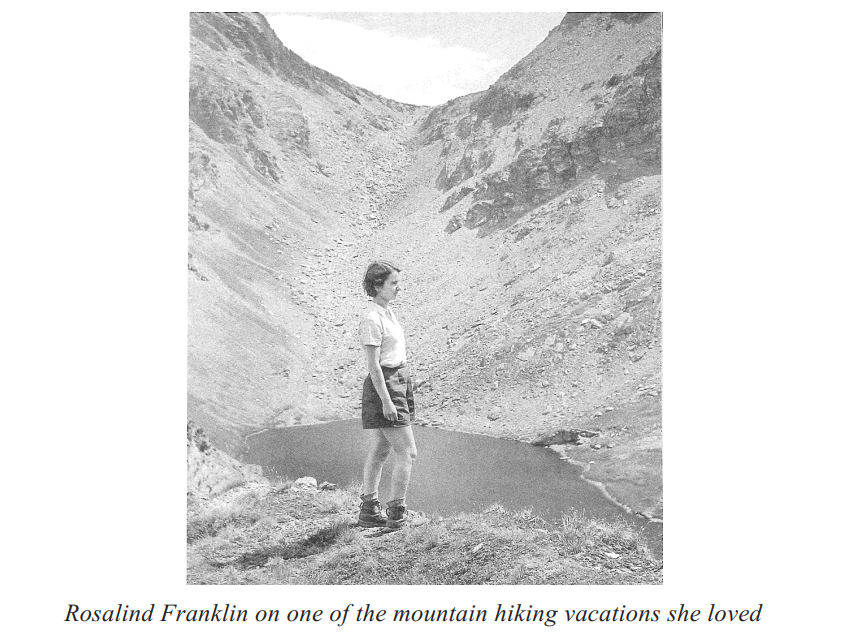
\includegraphics[width=0.75\linewidth]{image/Text5/Fig5.12.png}
\end{figure}

\noindent 33\\
Just back from a four - year X - ray crystallographic investigation of graphite in Paris, Franklin had been assigned to the DNA project while Wilkins was away from King’s. Unfortunately, the pair soon proved incompatible. Franklin, direct and data - focused, and Wilkins, retiring and speculative, were destined never to collaborate. Shortly before Wilkins accepted our lunch invitation, the two had had a big blowup in which Franklin had insisted that no model - building could commence before she collected much more extensive diffraction data. Now they effectively didn’t communicate, and Wilkins would have no chance to learn of her progress until Franklin presented her lab seminar scheduled for the beginning of November. If we wanted to listen, Crick and I were welcome to go as Wilkins’s guests.v
富兰克林刚结束在巴黎为期四年的石墨X射线晶体学研究回到英国,在威尔金斯离开伦敦国王学院期间,她被安排到了DNA研究项目中。不幸的是,两人很快就表现出合不来的情况。富兰克林直率且专注于数据,而威尔金斯内敛又喜欢推测,注定无法合作。就在威尔金斯接受我们的午餐邀请前不久,两人大吵了一架,富兰克林坚持在收集到更广泛的衍射数据之前,不能开始搭建模型。现在他们实际上不再交流,在富兰克林于11月初举办实验室研讨会之前,威尔金斯没有机会了解她的研究进展。如果我和克里克想听研讨会,可以作为威尔金斯的客人一同前往。\\

\noindent 34\\
Crick was unable to make the seminar, so I attended alone and briefed him later on what I believed to be its key take - home messages on crystalline DNA. In particular, I described from memory Franklin’s measurements of the crystallographic repeats and the water content. This prompted Crick to begin sketching helical grids on a sheet of paper, explaining that the new helical X - ray theory he had devised with Bill Cochran and Vladimir Vand would permit even me, a former bird - watcher, to predict correctly the diffraction patterns expected from the molecular models we would soon be building at the Cavendish.\\
克里克没能参加那场研讨会,所以我独自前往,之后我向他简要介绍了我认为这场研讨会中关于结晶DNA的关键要点。我还特别凭记忆描述了富兰克林对晶体学重复间距和含水量的测量结果。这促使克里克开始在纸上绘制螺旋网格,并解释说,他与比尔·科克伦和弗拉基米尔·万德共同提出的螺旋X射线新理论,即使是我这样一个曾经的观鸟爱好者,也能够正确预测我们即将在卡文迪许实验室搭建的分子模型的衍射图样。\\

\noindent 35\\
As soon as we got back to Cambridge, I arranged for the Cavendish machine shop to construct the phosphorous atom models needed for short sections of the sugar phosphate backbone found in DNA. Once these became available, we tested different ways the backbones might twist around each other in the center of the DNA molecule. Their regular repeating atomic structure should allow the atoms to come together in a consistent, repeated conformation. Following Wilkins’s hunch, we focused on three-chain models. When one of these appeared to be almost plausible, Crick made a phone call to Wilkins to announce we had a model we thought might be DNA.\\
我们一回到剑桥,我就安排卡文迪许实验室的机械车间制作DNA中磷酸核糖骨架短链段所需的磷原子模型。模型一做好,我们就测试了这些骨架在DNA分子中心相互缠绕的不同方式。其规则重复的原子结构应能使原子以一致且重复的构象聚集在一起。根据威尔金斯的直觉,我们专注于三链模型。当其中一个模型看起来几乎可行时,克里克打电话给威尔金斯,说我们搭建出了一个认为可能是DNA结构的模型。\\

\noindent 36\\
The next day both Wilkins and Franklin came up to see what we had done. The threat of unanticipated competition briefly united them in common purpose. Franklin wasted no time in faulting our basic concept. My memory was that she had reported almost no water present in crystalline DNA. In fact, the opposite was true. Being a crystallographic novice, I had confused the terms “unit cell” and “asymmetric unit.” Crystalline DNA was in fact water-rich. Consequently, Franklin pointed out, the backbone had to be on the outside and not, as we had it, in the center, if only to accommodate all the water molecules she had observed in her crystals.\\
第二天,威尔金斯和富兰克林都过来看我们的成果。未曾预料到的竞争带来的威胁,让他们在短时间内有了共同目标。富兰克林立刻指出了我们基本构想中的问题。我记得她曾报告说结晶DNA中几乎不含水,而事实恰恰相反。作为晶体学新手,我混淆了 “晶胞” 和 “不对称单位” 这两个术语。实际上,结晶DNA富含水分。因此,富兰克林指出,为了容纳她在晶体中观察到的所有水分子,磷酸 - 脱氧核糖骨架必须位于外侧,而不是像我们所设想的那样位于中心。\\

\noindent 37\\
That unfortunate November day cast a very long shadow. Franklin’s opposition to model-building was reinforced. Doing experiments, not playing with Tinkertoy representations of atoms, was the way she intended to proceed. Even worse, Sir Lawrence Bragg passed down the word that Crick and I should desist from all further attempts at building a DNA model. It was further decreed that DNA research should be left to the King’s lab, with Cambridge continuing to focus solely on proteins. There was no sense in two MRC-funded labs competing against each other. With no more bright ideas up our sleeves, Crick and I were reluctantly forced to back off, at least for the time being.\\
那个不幸的11月的日子带来了长久的影响。富兰克林更加反对搭建模型了。她打算通过做实验,而不是摆弄原子模型来开展研究。更糟糕的是,劳伦斯·布拉格爵士传话下来,让我和克里克停止一切进一步搭建DNA模型的尝试。他还下令DNA研究应该由伦敦国王学院的实验室负责,剑桥这边继续只专注于蛋白质研究。两个由医学研究委员会资助的实验室相互竞争毫无意义。由于我们也没有新的好主意,我和克里克只好不情愿地暂时放弃。\\

\noindent 38\\
It was not a good moment to be condemned to the DNA sidelines. Linus Pauling had written Wilkins to request a copy of the crystalline DNA diffraction pattern. Though Wilkins had declined, saying he wanted more time to interpret it himself, Pauling was hardly obliged to depend upon data from King’s. If he wished, he could easily start serious X-ray diffraction studies at Caltech.\\
被排除在DNA研究之外可不是个好时候。莱纳斯·鲍林写信给威尔金斯,索要一份结晶DNA的衍射图谱。尽管威尔金斯拒绝了,称自己还需要更多时间来分析图谱,但鲍林并非只能依靠国王学院的数据。如果他愿意,他可以很容易地在加州理工学院开展严谨的X射线衍射研究。\\

\noindent 39\\
The following spring, I duly turned away from DNA and set about extending prewar studies on the pencil-shaped tobacco mosaic virus using the Cavendish’s powerful new X-ray beam. This light experimental workload gave me plenty of time to wander through various Cambridge libraries. In the zoology building, I read Erwin Chargaff’s paper describing his finding that the DNA bases adenine and thymine occurred in roughly equal amounts, as did the bases guanine and cytosine. Hearing of these one-to-one ratios Crick wondered whether, during DNA duplication, adenine residues might be attracted to thymine and vice versa, and whether a corresponding attraction might exist between guanine and cytosine. If so, base sequences on the “parental” chains (e.g., ATGC) would have to be complementary to those on “daughter” strands (yielding in this case TACG). \\
第二年春天,我顺从地放下了DNA研究,开始利用卡文迪许实验室强大的新型X射线束,拓展对铅笔状烟草花叶病毒的战前研究。实验任务不重,这让我有大量时间流连于剑桥的各个图书馆。在动物学楼里,我读到了埃尔文·查戈夫的论文,他在文中描述了自己的发现:DNA中的腺嘌呤和胸腺嘧啶的含量大致相等,鸟嘌呤和胞嘧啶的含量也是如此。听到这些碱基一一对应的比例关系后,克里克猜想,在DNA复制过程中,腺嘌呤残基是否会被胸腺嘧啶吸引,反之亦然,以及鸟嘌呤和胞嘧啶之间是否也存在类似的吸引关系。如果是这样, “亲代” 链上的碱基序列(例如ATGC)就必须与 “子代” 链上的互补(在这种情况下是TACG)。\\ 

\noindent 40\\
These remained idle thoughts until Erwin Chargaff came through Cambridge in the summer of 1952 on his way to the International Biochemical Congress in Paris. Chargaff expressed annoyance that neither Crick nor I saw the need to know the chemical structures of the four bases. He was even more upset when we told him that we could simply look up the structures in textbooks as the need arose. I was left hoping that Chargaff’s data would prove irrelevant. Crick, however, was energized to do several experiments looking for molecular “sandwiches” that might form when adenine and thymine (or alternatively, guanine and cytosine) were mixed together in solution. But his experiments went nowhere.\\
这些想法一直停留在空想阶段,直到1952年夏天埃尔文·查戈夫途经剑桥前往巴黎参加国际生物化学大会。查戈夫很恼火,因为我和克里克都觉得没必要了解四种碱基的化学结构。当我们告诉他,有需要时我们可以直接在教科书里查阅这些结构时,他更生气了。我暗自希望查戈夫的数据被证明是无关紧要的。然而,克里克却充满干劲地做了几个实验,试图找出腺嘌呤和胸腺嘧啶(或者鸟嘌呤和胞嘧啶)在溶液中混合时可能形成的分子 “夹层” 结构,但他的实验毫无进展。 \\

\noindent 41\\
Like Chargaff, Linus Pauling also attended the International Biochemical Congress, where the big news was the latest result from the Phage Group. Alfred Hershey and Martha Chase at Cold Spring Harbor had just confirmed Avery’s transforming principle: DNA was the hereditary material! Hershey and Chase proved that only the DNA of the phage virus enters bacterial cells; its protein coat remains on the outside. It was more obvious than ever that DNA must be understood at the molecular level if we were to uncover the essence of the gene. With Hershey and Chase’s result the talk of the town, I was sure that Pauling would now bring his formidable intellect and chemical wisdom to bear on the problem of DNA.\\
和查戈夫一样,莱纳斯·鲍林也参加了国际生物化学大会,大会上的重大新闻是噬菌体小组的最新研究成果。冷泉港实验室的阿尔弗雷德·赫尔希和玛莎·蔡斯刚刚证实了艾弗里的转化原理:DNA是遗传物质!赫尔希和蔡斯证明,只有噬菌体病毒的DNA会进入细菌细胞,其蛋白质外壳则留在细胞外。现在比以往任何时候都更明显的是,如果我们想要揭示基因的本质,就必须从分子层面去理解DNA。赫尔希和蔡斯的研究成果成了人们热议的话题,我确信鲍林现在会运用他卓越的智慧和化学知识来研究DNA问题。\\

\noindent 42\\
Early in 1953, Pauling did indeed publish a paper outlining the structure of DNA. Reading it anxiously I saw that he was proposing a three-chain model with sugar phosphate backbones forming a dense central core. Superficially it was similar to our botched model of fifteen months earlier. But instead of using positively charged atoms (e.g., Mg²⁺) to stabilize the negatively charged backbones, Pauling made the unorthodox suggestion that the phosphates were held together by hydrogen bonds. But it seemed to me, the biologist, that such hydrogen bonds required extremely acidic conditions never found in cells. With a mad dash to Alexander Todd’s nearby organic chemistry lab my belief was confirmed: The impossible had happened. The world’s best-known, if not best, chemist had gotten his chemistry wrong. In effect, Pauling had knocked the A off of DNA. Our quarry was deoxyribonucleic acid, but the structure he was proposing was not even acidic.\\
1953年初,鲍林确实发表了一篇概述DNA结构的论文。我急切地读完后发现,他提出了一个三链模型,其中磷酸核糖骨架形成一个致密的核心。从表面上看,这与我们15个月前失败的模型相似。但鲍林没有使用带正电的原子(如镁离子Mg²⁺)来稳定带负电的骨架,而是提出了一个非传统的观点,即磷酸盐是通过氢键结合在一起的。但在我这个生物学家看来,这种氢键的形成需要细胞中不存在的强酸性条件。我急忙跑到附近亚历山大·托德的有机化学实验室,证实了我的想法:不可能的事情发生了。这位世界上最知名(即便不是最优秀)的化学家在化学问题上出错了。实际上,鲍林颠覆了DNA中的 “酸(acid)” 这一概念。我们要研究的是脱氧核糖核酸,但他提出的结构甚至都不具备酸性。\\

\noindent 43\\
Hurriedly I took the manuscript to London to inform Wilkins and Franklin they were still in the game. Convinced that DNA was not a helix, Franklin had no wish even to read the article and deal with the distraction of Pauling’s helical ideas, even when I offered Crick’s arguments for helices. Wilkins, however, was very interested indeed in the news I brought; he was now more certain than ever that DNA was helical. To prove the point, he showed me a photograph obtained more than six months earlier by Franklin’s graduate student Raymond Gosling, who had X-rayed the so-called B form of DNA. Until that moment, I didn’t know a B form even existed. Franklin had put this picture aside, preferring to concentrate on the A form, which she thought would more likely yield useful data. The X-ray pattern of this B form was a distinct cross. Since Crick and others had already deduced that such a pattern of reflections would be created by a helix, this evidence made it clear that DNA had to be a helix! In fact, despite Franklin’s reservations, this was no surprise. Geometry itself suggested that a helix was the most logical arrangement for a long string of repeating units such as the nucleotides of DNA. But we still did not know what that helix looked like, nor how many chains it contained.\\
我匆忙带着这份手稿前往伦敦,告诉威尔金斯和富兰克林,他们仍有机会在DNA结构研究上取得成果。富兰克林坚信DNA不是螺旋结构,甚至不愿去读鲍林的那篇文章,也不想理会鲍林有关螺旋结构的观点,即便我提出了克里克支持螺旋结构的论据。然而,威尔金斯对我带来的消息非常感兴趣,他比以往任何时候都更加确信DNA是螺旋形的。为了证明这一点,他给我看了一张照片,那是富兰克林的研究生雷蒙德·戈斯林在六个多月前拍摄的,是对所谓的B型DNA进行X射线衍射的结果。在那之前,我甚至都不知道还有B型DNA的存在。富兰克林把这张照片搁置了,她更倾向于专注研究A型DNA,认为其更有可能产生有用的数据。B型DNA的X射线衍射图谱呈现出一个清晰的十字形。由于克里克和其他人此前已经推断出,这样的衍射图谱是由螺旋结构产生的,所以这一证据清楚地表明,DNA必定是螺旋结构!事实上,尽管富兰克林持保留意见,但这并不意外。从几何学角度来看,对于像DNA中的核苷酸这样一长串重复单元而言,螺旋结构是最合理的排列方式。但我们仍然不知道这个螺旋结构是什么样子,也不清楚它包含多少条链。\\ 

\noindent 44\\
The time had come to resume building helical models of DNA. Pauling was bound to realize soon enough that his brainchild was wrong. I urged Wilkins to waste no time. But he wanted to wait until Franklin had completed her scheduled departure for another lab later that spring. She had decided to move on to avoid the unpleasantness at King’s. Before leaving, she had been ordered to stop further work with DNA and had already passed on many of her diffraction images to Wilkins.\\
是时候重新开始搭建DNA的螺旋结构模型了。鲍林很快就会意识到,他的心血之作是错误的。我催促威尔金斯不要浪费时间。但他想等到富兰克林在那年春天晚些时候按计划离开,前往另一个实验室之后再说。她为了避免在伦敦国王学院的不愉快而决定离开。在离开之前,她被要求停止DNA相关的进一步研究工作,并且已经把自己的许多衍射图像交给了威尔金斯。\\

\begin{figure}
    \centering
    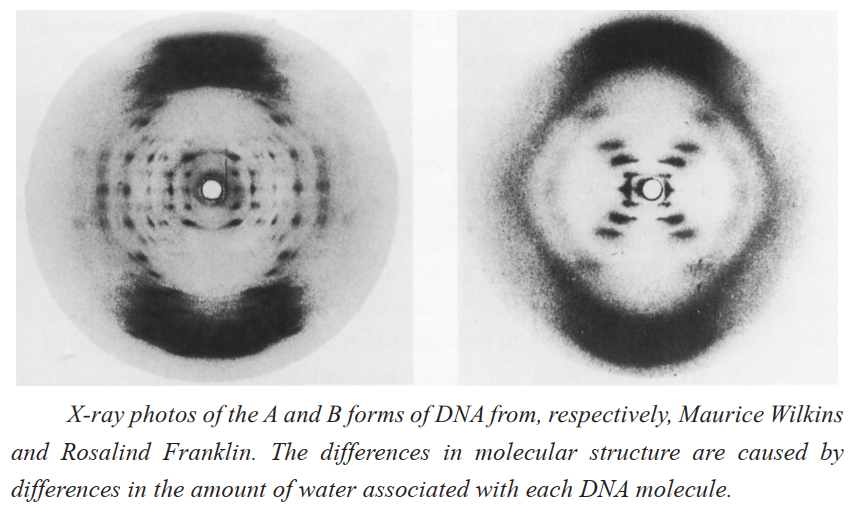
\includegraphics[width=0.75\linewidth]{image/Text5/Fig5.13.png}
\end{figure}

\noindent 45\\
When I returned to Cambridge and broke the news of the DNA B form, Bragg no longer saw any reason for Crick and me to avoid DNA. He very much wanted the DNA structure to be found on his side of the Atlantic. So we went back to model - building, looking for a way the known basic components of DNA—the backbone of the molecule and the four different bases, adenine, thymine, guanine, and cytosine—could fit together to make a helix. I commissioned the shop at the Cavendish to make us a set of tin bases, but they couldn’t produce them fast enough for me: I ended up cutting out rough approximations from stiff cardboard.\\
我回到剑桥,把发现DNA B型结构的消息告知大家后,布拉格认为我和克里克没有理由再避开DNA研究了。他非常希望能由大西洋这边(即英国)的团队发现DNA的结构。于是我们重新开始搭建模型,试图找到一种方式,将已知的DNA基本组成部分——分子骨架以及腺嘌呤、胸腺嘧啶、鸟嘌呤和胞嘧啶这四种不同的碱基——组合在一起,形成螺旋结构。我请卡文迪许实验室的车间制作一套金属碱基模型,但他们的制作速度无法满足我的需求,最后我只好用硬纸板剪出大致的模型。\\

\noindent 46\\
By this time I realized the DNA density-measurement evidence actually slightly favored a two-chain, rather than three-chain, model. So I decided to search out plausible double helices. As a biologist, I preferred the idea of a genetic molecule made of two, rather than three, components. After all, chromosomes, like cells, increase in number by duplicating, not triplicating.
这时我意识到,DNA密度测量的证据实际上更倾向于双链模型,而非三链模型。所以我决定寻找合理的双螺旋结构。作为一名生物学家,我更倾向于遗传分子由两部分组成,而不是三部分。毕竟,染色体和细胞一样,是通过复制(加倍)而非 “复制三倍” 来增加数量的。\\

\begin{figure}
    \centering
    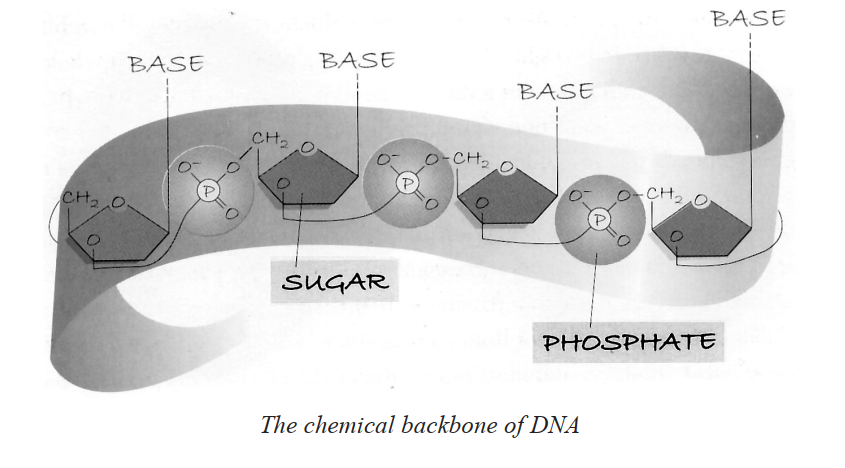
\includegraphics[width=0.75\linewidth]{image/Text5/Fig5.14.png}
\end{figure}

\noindent 47\\
I knew that our previous model with the backbone on the inside and the bases hanging out was wrong. Chemical evidence from the University of Nottingham, which I had too long ignored, indicated that the bases must be hydrogen-bonded to each other. They could only form bonds like this in the regular manner implied by the X-ray diffraction data if they were in the center of the molecule. But how could they come together in pairs? For two weeks I got nowhere, misled by an error in my nucleic acid chemistry textbook. Happily, on February 27, Jerry Donahue, a theoretical chemist visiting the Cavendish from Caltech, pointed out that the textbook was wrong. So I changed the locations of the hydrogen atoms on my cardboard cutouts of the molecules.\\
我知道,我们之前提出的磷酸 - 脱氧核糖骨架在内、碱基在外的模型是错误的。诺丁汉大学的化学研究证据表明,碱基之间必定存在氢键,而我此前一直忽视了这一点。根据X射线衍射数据显示,如果碱基位于分子中心,它们才能以规律的方式形成这样的化学键。但它们如何成对结合呢?有两周时间,我毫无进展,被核酸化学教科书里的一个错误误导了。幸运的是,2月27日,从加州理工学院到卡文迪许实验室访问的理论化学家杰里·多纳休指出了教科书里的错误。于是我更改了用硬纸板剪出的分子模型上氢原子的位置。 \\

\noindent 48\\
The next morning, February 28, 1953, the key features of the DNA model all fell into place. The two chains were held together by strong hydrogen bonds between adenine-thymine and guanine-cytosine base pairs. The inferences Crick had drawn the year before based on Chargaff’s research had indeed been correct. Adenine does bond to thymine and guanine does bond to cytosine, but not through flat surfaces to form molecular sandwiches. When Crick arrived, he took it all in rapidly, and gave my base-pairing scheme his blessing. He realized right away that it would result in the two strands of the double helix running in opposite directions.\\
第二天早上,也就是1953年2月28日,DNA模型的关键特征都确定下来了。两条链通过腺嘌呤 - 胸腺嘧啶以及鸟嘌呤 - 胞嘧啶碱基对之间的强氢键结合在一起。克里克前一年基于查戈夫的研究所得出的推论确实是正确的。腺嘌呤与胸腺嘧啶结合,鸟嘌呤与胞嘧啶结合,但不是通过平面形成分子 “夹层” 结构。克里克到了之后,很快理解了整个模型,并认可了我的碱基配对方案。他立刻意识到,这会使得双螺旋的两条链方向相反。 \\

\noindent 49\\
It was quite a moment. We felt sure that this was it. Anything that simple, that elegant just had to be right. What got us most excited was the complementarity of the base sequences along the two chains. If you knew the sequence—the order of bases—along one chain, you automatically knew the sequence along the other. It was immediately apparent that this must be how the genetic messages of genes are copied so exactly when chromosomes duplicate prior to cell division. The molecule would “unzip” to form two separate strands. Each separate strand then could serve as the template for the synthesis of a new strand, one double helix becoming two.\\
那真是一个激动人心的时刻。我们确信就是它了。如此简单而又精妙的结构,必定是正确的。最让我们兴奋的是两条链上碱基序列的互补性。如果你知道一条链上的碱基序列,就能自然而然地知道另一条链上的序列。很明显,这一定就是在细胞分裂前染色体复制时,基因的遗传信息能够精确复制的方式。DNA分子会 “解旋” 形成两条单链,随后每条单链都可以作为合成新链的模板,一个双螺旋结构就变成了两个。 \\

\noindent 50\\
In *What is Life?* Schrödinger had suggested that the language of life might be like Morse code, a series of dots and dashes. He wasn’t far off. The language of DNA is a linear series of As, Ts, Gs, and Cs. And just as transcribing a page out of a book can result in the odd typo, the rare mistake creeps in when all these As, Ts, Gs, and Cs are being copied along a chromosome. These errors are the mutations geneticists had talked about for almost fifty years. Change an “i” to an “a” and “Jim” becomes “Jam” in English; change a T to a C and “ATG” becomes “ACG” in DNA.\\
在《生命是什么?》一书中,薛定谔曾提出,生命的语言可能就像摩尔斯电码,由一系列的点和划组成。他的想法相差不远。DNA的 “语言” 是由腺嘌呤(A)、胸腺嘧啶(T)、鸟嘌呤(G)和胞嘧啶(C)组成的线性序列。就像抄写书中的一页内容可能会出现偶尔的拼写错误一样,当这些A、T、G和C在染色体中被复制时,也会偶尔出现罕见的错误。这些错误就是遗传学家们近五十年来一直在讨论的突变。在英语中,把 “i” 改成 “a”,“Jim” 就变成了 “Jam” ;在DNA中,把T改成C,“ATG” 就变成了 “ACG”。 \\

\begin{figure}
    \centering
    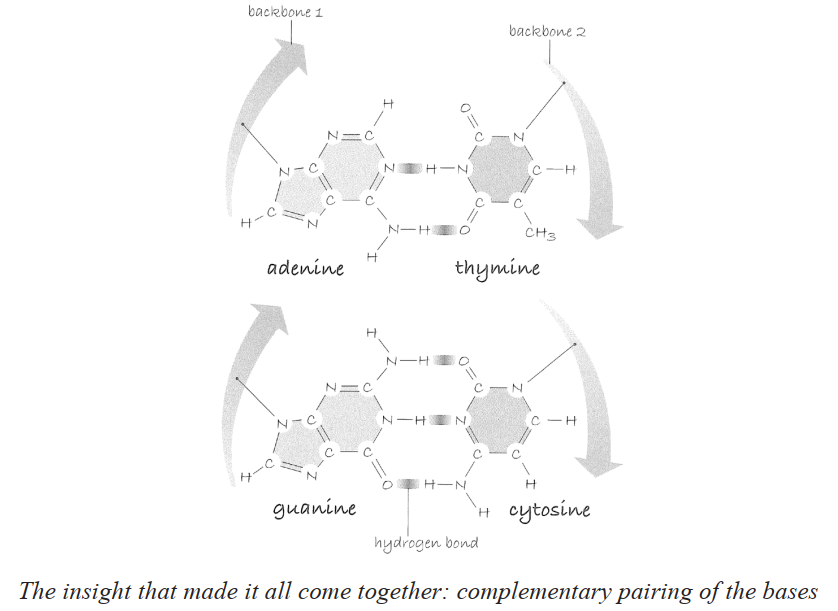
\includegraphics[width=0.75\linewidth]{image/Text5/Fig5.15.png}
\end{figure}

\begin{figure}
    \centering
    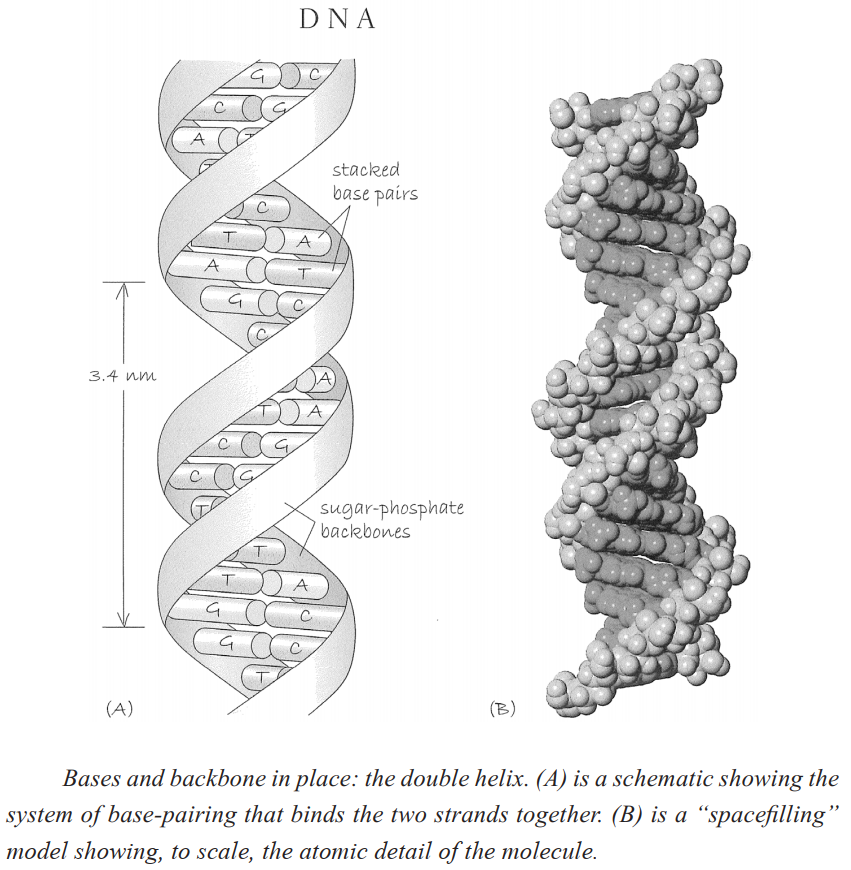
\includegraphics[width=0.75\linewidth]{image/Text5/Fig5.16.png}
\end{figure}

\noindent 51\\
The double helix made sense chemically and it made sense biologically. Now there was no need to be concerned about Schrödinger’s suggestion that new laws of physics might be necessary for an understanding of how the hereditary code-script is duplicated: genes in fact were no different from the rest of chemistry. Later that day, during lunch at the Eagle, the pub virtually adjacent to the Cavendish Lab, Crick, ever the talker, could not help but tell everyone we had just found the “secret of life.” I myself, though no less electrified by the thought, would have waited until we had a pretty three-dimensional model to show off.\\
DNA双螺旋结构在化学和生物学上都有其合理性。现在,也无需担心薛定谔曾提出的观点,即可能需要新的物理定律来解释遗传密码是如何复制的:事实上,基因与其他化学物质并无不同。那天晚些时候,在卡文迪许实验室附近的老鹰酒吧吃午饭时,一向健谈的克里克忍不住告诉每个人,我们刚刚发现了 “生命的奥秘” 。而我自己,虽然同样为此兴奋不已,但本想等到做出一个精美的三维模型后再炫耀。 \\

\noindent 52\\
Among the first to see our demonstration model was the chemist Alexander Todd. That the nature of the gene was so simple both surprised and pleased him. Later, however, he must have asked himself why his own lab, having established the general chemical structure of DNA chains, had not moved on to asking how the chains folded up in three dimensions. Instead the essence of the molecule was left to be discovered by a two - man team, a biologist and a physicist, neither of whom possessed a detailed command even of undergraduate chemistry. But paradoxically, this was, at least in part, the key to our success: Crick and I arrived at the double helix first precisely because most chemists at that time thought DNA too big a molecule to understand by chemical analysis.\\
最早看到我们演示模型的人之一是化学家亚历山大·托德。基因的本质如此简单,这既让他感到惊讶,又让他欣喜。然而,后来他肯定反思过,为什么自己的实验室在确定了DNA链的一般化学结构后,却没有进一步研究这些链是如何折叠成三维结构的。最终,这个分子的奥秘却是由一个两人团队发现的,团队成员一个是生物学家,一个是物理学家,他们甚至都没有全面掌握本科化学知识。但矛盾的是,这至少在一定程度上是我们成功的关键:我和克里克之所以能率先发现双螺旋结构,恰恰是因为当时大多数化学家都认为DNA分子太大,无法通过化学分析来理解 。 \\

\noindent 53\\
At the same time, the only two chemists with the vision to seek DNA’s 3-D structure made major tactical mistakes: Rosalind Franklin’s was her resistance to model-building; Linus Pauling’s was a matter of simply neglecting to read the existing literature on DNA, particularly the data on its base composition published by Chargaff. Ironically, Pauling and Chargaff sailed across the Atlantic on the same ship following the Paris Biochemical Congress in 1952, but failed to hit it off. Pauling was long accustomed to being right. And he believed there was no chemical problem he could not work out from first principles by himself. Usually this confidence was not misplaced. During the Cold War, as a prominent critic of the American nuclear weapons development program, he was questioned by the FBI after giving a talk. How did he know how much plutonium there is in an atomic bomb? Pauling’s response was “Nobody told me. I figured it out.”\\
与此同时,仅有的两位有远见去探寻DNA三维结构的化学家都犯了重大的策略性错误:罗莎琳德·富兰克林的错误在于她抵触搭建模型;莱纳斯·鲍林的问题则是完全忽视了阅读现有的关于DNA的文献,特别是查戈夫发表的有关DNA碱基组成的数据。具有讽刺意味的是,1952年巴黎生物化学大会之后,鲍林和查戈夫同船穿越大西洋,但两人却没能谈得来。鲍林长期以来习惯了自己总是正确的。他相信没有什么化学问题是他不能从基本原理出发独自解决的。通常情况下,这种自信并非毫无根据。冷战期间,作为美国核武器发展计划的著名批评者,他在一次演讲后被美国联邦调查局讯问。他们问他是怎么知道一颗原子弹里有多少钚的,鲍林回答说:“没人告诉我,我自己算出来的。” \\

\noindent 54\\
Over the next several months Crick and (to a lesser extent) I relished showing off our model to an endless stream of curious scientists. However, the Cambridge biochemists did not invite us to give a formal talk in the biochemistry building. They started to refer to it as the “WC,” punning our initials with those used in Britain for the toilet or water closet. That we had found the double helix without doing experiments irked them.\\
在接下来的几个月里,克里克以及我(相对少一些)乐于向源源不断的好奇科学家展示我们的模型。然而,剑桥的生物化学家们没有邀请我们在生物化学楼里进行正式演讲。他们开始戏称这个模型为 “WC”,这是拿我们姓氏的首字母和英国表示厕所的缩写玩双关。我们没做实验就发现了双螺旋结构,这让他们很恼火。\ 

\noindent 55\\
The manuscript that we submitted to *Nature* in early April was published just over three weeks later, on April 25, 1953. Accompanying it were two longer papers by Franklin and Wilkins, both supporting the general correctness of our model. In June, I gave the first presentation of our model at the Cold Spring Harbor symposium on viruses. Max Delbrück saw to it that I was offered, at the last minute, an invitation to speak. To this intellectually high-powered meeting I brought a three-dimensional model built in the Cavendish, the adenine-thymine base pairs in red and the guanine-cytosine base pairs in green.\\
我们在4月初提交给《自然》杂志的论文,在三周多一点后的1953年4月25日发表了。一同发表的还有富兰克林和威尔金斯的两篇篇幅更长的论文,他们都认可我们提出的DNA模型在总体上是正确的。6月,我在冷泉港病毒研讨会上首次介绍了我们的模型。马克斯·德尔布吕克安排我在最后一刻得到了发言邀请。在这场学术大咖云集的会议上,我展示了一个在卡文迪许实验室制作的三维模型,其中腺嘌呤 - 胸腺嘧啶碱基对是红色的,鸟嘌呤 - 胞嘧啶碱基对是绿色的。 \\

\begin{figure}
    \centering
    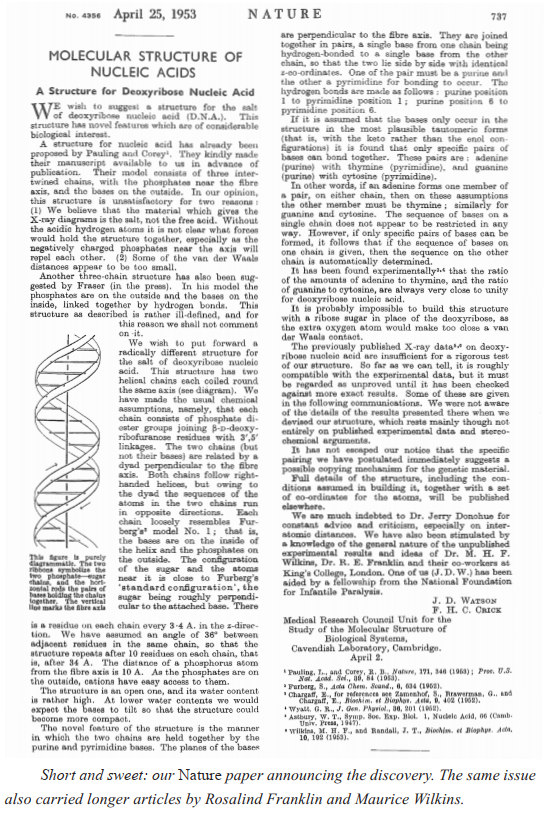
\includegraphics[width=0.75\linewidth]{image/Text5/Fig5.17.png}
\end{figure}

\begin{figure}
    \centering
    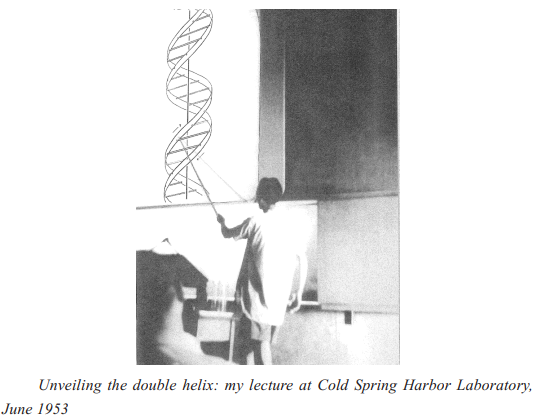
\includegraphics[width=0.75\linewidth]{image/Text5/Fig5.18.png}
\end{figure}

\noindent 56\\
In the audience was Seymour Benzer, yet another ex - physicist who had heeded the clarion call of Schrödinger’s book. He immediately understood what our breakthrough meant for his studies of mutations in viruses. He realized that he could now do for a short stretch of bacteriophage DNA what Morgan’s boys had done forty years earlier for fruit fly chromosomes: he would map mutations—determine their order—along a gene, just as the fruit fly pioneers had mapped genes along a chromosome. Like Morgan, Benzer would have to depend on recombination to generate new genetic combinations, but, whereas Morgan had the advantage of a ready mechanism of recombination—the production of sex cells in a fruit fly—Benzer had to induce recombination by simultaneously infecting a single bacterial host cell with two different strains of bacteriophage, which differed by one or more mutations in the region of interest. Within the bacterial cell, recombination—the exchange of segments of molecules—would occasionally occur between the different viral DNA molecules, producing new permutations of mutations—so - called “recombinants.” Within a single astonishingly productive year in his Purdue University lab, Benzer produced a map of a single bacteriophage gene, *rII*, showing how a series of mutations—all errors in the genetic script—were laid out linearly along the virus DNA. The language was simple and linear, just like a line of text on the written page.\\
听众中有西摩·本泽,他也是一位从前的物理学家,曾响应薛定谔著作的号召转行。他立刻明白我们的突破对他研究病毒突变意味着什么。他意识到,现在他可以在一小段噬菌体DNA上做四十年前摩根的团队在果蝇染色体上所做的事:他将绘制突变图谱,确定基因上突变的顺序,就像果蝇研究的先驱们绘制染色体上的基因图谱一样。和摩根一样,本泽得依靠基因重组来产生新的基因组合,但摩根有现成的重组机制(果蝇产生性细胞的过程)这一优势,而本泽则必须用两种不同的噬菌体菌株同时感染单个细菌宿主细胞来诱导重组,这两种菌株在目标区域存在一处或多处突变差异。在细菌细胞内,不同的病毒DNA分子之间偶尔会发生重组(即分子片段的交换),从而产生突变的新排列组合,也就是所谓的 “重组体” 。在普渡大学实验室,本泽在成果惊人的短短一年时间里,绘制出了单个噬菌体基因*rII*的图谱,展示了一系列突变(即遗传密码中的错误)是如何沿病毒DNA呈线性排列的。这种 “语言” 简单而线性,就像书面上的一行文字 。 \\

\noindent 57\\
The response of the Hungarian physicist Leo Szilard to my Cold Spring Harbor talk on the double helix was less academic. His question was, “Can you patent it?” At one time Szilard’s main source of income had been a patent that he held with Einstein, and he had later tried unsuccessfully to patent with Enrico Fermi the nuclear reactor they built at the University of Chicago in 1942. But then as now patents were given only for useful inventions and at the time no one could conceive of a practical use for DNA. Perhaps then, Szilard suggested, we should copyright it.\\
匈牙利物理学家利奥·西拉德对我在冷泉港关于DNA双螺旋结构的演讲的反应没那么学术。他的问题是:“你能为它申请专利吗?” 西拉德曾有段时间的主要收入来源,是他和爱因斯坦共同持有的一项专利,后来他还试图与恩里科·费米就1942年他们在芝加哥大学建造的核反应堆申请专利,但没有成功。当时和现在一样,专利只授予有用的发明,而那时没人能想到DNA的实际用途。于是西拉德建议,也许我们应该为它申请版权。\\

\begin{figure}
    \centering
    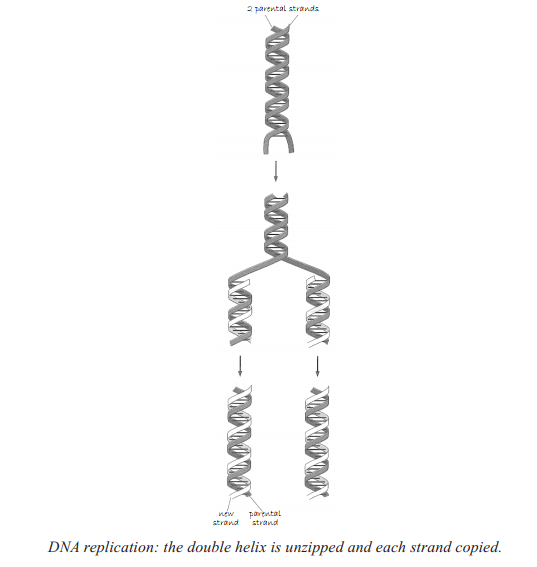
\includegraphics[width=0.75\linewidth]{image/Text5/Fig5.19.png}
\end{figure}

\noindent 58\\
There remained, however, a single missing piece in the double helical jigsaw puzzle: our unzipping idea for DNA replication had yet to be experimentally verified. Max Delbrück, for example, was unconvinced. Though he liked the double helix as a model, he worried that unzipping it might generate horrible knots. Five years later, a former student of Pauling’s, Matt Meselson, and the equally bright young phage worker Frank Stahl put to rest such fears when they published the results of a single elegant experiment.\\
然而,在DNA双螺旋结构这个拼图中仍缺少一块:我们提出的DNA复制时 “解旋” 的观点尚未得到实验验证。例如,马克斯·德尔布吕克就对此表示怀疑。尽管他认可双螺旋模型,但担心解旋过程中可能会产生复杂的纽结。五年后,鲍林以前的学生马特·梅塞尔森,以及同样聪慧的年轻噬菌体研究者弗兰克·斯塔尔,发表了一个巧妙的实验结果,打消了人们的这种担忧。 \\

\noindent 59\\
They had met in the summer of 1954 at the Marine Biological Laboratory at Woods Hole, Massachusetts, where I was then lecturing, and agreed—over a good many gin martinis—that they should get together to do some science. The result of their collaboration has been described as “the most beautiful experiment in biology.”
1954年夏天,他们在马萨诸塞州伍兹霍尔的海洋生物实验室相遇,当时我正在那里讲学。在喝了很多杯杜松子马提尼酒后,他们达成一致,认为应该携手开展一些科学研究。他们合作的成果被称为 “生物学中最精妙的实验”。 \\

\begin{figure}
    \centering
    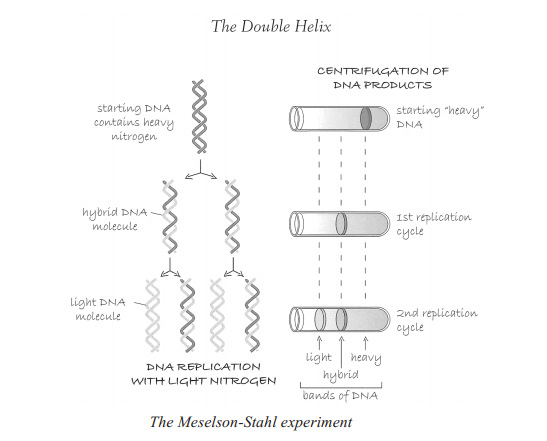
\includegraphics[width=0.75\linewidth]{image/Text5/Fig5.20.png}
\end{figure}

\noindent 60\\
They used a centrifugation technique that allowed them to sort molecules according to slight differences in weight; following a centrifugal spin, heavier molecules end up nearer the bottom of the test tube than lighter ones. Because nitrogen atoms (N) are a component of DNA, and because they exist in two distinct forms, one light and one heavy, Meselson and Stahl were able to tag segments of DNA and thereby track the process of its replication in bacteria. Initially all the bacteria were raised in a medium containing heavy N, which was thus incorporated in both strands of the DNA. From this culture they took a sample, transferring it to a medium containing only light N, ensuring that the next round of DNA replication would have to make use of light N. If, as Crick and I had predicted, DNA replication involves unzipping the double helix and copying each strand, the resultant two “daughter” DNA molecules in the experiment would be hybrids, each consisting of one heavy N strand (the template strand derived from the “parent” molecule) and one light N strand (the one newly fabricated from the new medium). Meselson and Stahl’s centrifugation procedure bore out these expectations precisely. They found three discrete bands in their centrifuge tubes, with the heavy-then-light sample halfway between the heavy-heavy and light-light samples. DNA replication works just as our model supposed it would.\\
他们采用了一种离心技术,该技术能根据分子重量的细微差异对其进行分离;经过离心旋转后,较重的分子会比较轻的分子更靠近试管底部。由于氮原子(N)是DNA的组成成分,且有两种不同的形式,即轻氮和重氮,梅塞尔森和斯塔尔得以标记DNA片段,进而追踪其在细菌中的复制过程。起初,所有细菌都在含有重氮的培养基中培养,因此重氮被整合到了DNA的两条链中。他们从该培养物中取出一份样本,转移到只含轻氮的培养基中,以确保下一轮DNA复制必须使用轻氮。正如我和克里克所预测的那样,如果DNA复制涉及双螺旋解旋以及每条链的复制,那么实验中产生的两个 “子代” DNA分子将是杂合分子,每个子代分子都由一条重氮链(来自 “亲代” 分子的模板链)和一条轻氮链(在新培养基中新合成的链)组成。梅塞尔森和斯塔尔的离心实验结果完全证实了这些预期。他们在离心管中发现了三条清晰的条带,先重后轻的样本条带位于全重样本条带和全轻样本条带的中间位置。DNA的复制过程正如我们的模型所设想的那样。\\ 

\begin{figure}
    \centering
    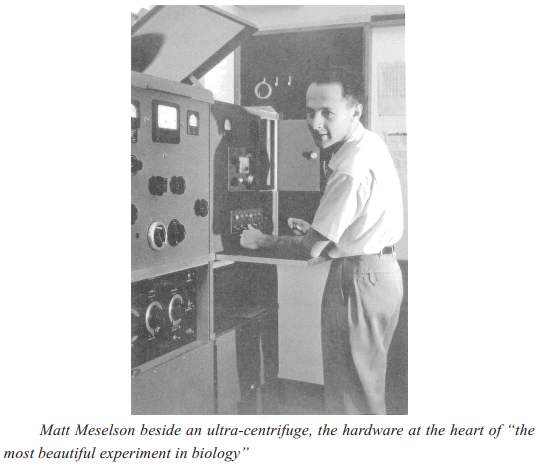
\includegraphics[width=0.75\linewidth]{image/Text5/Fig5.21.png}
\end{figure}

\noindent 61\\
The biochemical nuts and bolts of DNA replication were being analyzed at around the same time in Arthur Kornberg’s laboratory at Washington University in St. Louis. By developing a new, “cell-free” system for DNA synthesis, Kornberg discovered an enzyme (DNA polymerase) that links the DNA components and makes the chemical bonds of the DNA backbone. Kornberg’s enzymatic synthesis of DNA was such an unanticipated and important event that he was awarded the 1959 Nobel Prize in Physiology or Medicine, less than two years after the key experiments. After his prize was announced, Kornberg was photographed holding a copy of the double helix model I had taken to Cold Spring Harbor in 1953.\\
大约在同一时期,圣路易斯华盛顿大学亚瑟·科恩伯格的实验室正在对DNA复制的生物化学基本原理进行分析。科恩伯格通过开发一种新的 “无细胞” DNA合成系统,发现了一种酶(DNA聚合酶),这种酶可以连接DNA的各个组成部分,并形成DNA骨架的化学键。科恩伯格在酶作用下进行的DNA合成是一项出乎意料的重大发现,在关键实验完成后不到两年,他就被授予了1959年诺贝尔生理学或医学奖。在宣布他获奖之后,有人拍到他手持一个我于1953年带到冷泉港的双螺旋结构模型复制品。\\

\noindent 62\\
It was not until 1962 that Francis Crick, Maurice Wilkins, and I were to receive our own Nobel Prize in Physiology or Medicine. Four years earlier, Rosalind Franklin had died of ovarian cancer at the tragically young age of thirty-seven. Before then Crick had become a close colleague and a real friend of Franklin’s. Following the two operations that would fail to stem the advance of her cancer, Franklin convalesced with Crick and his wife, Odile, in Cambridge.\\
直到1962年,弗朗西斯·克里克、莫里斯·威尔金斯和我才获得诺贝尔生理学或医学奖。四年前,罗莎琳德·富兰克林因卵巢癌去世,年仅37岁,令人惋惜。在此之前,克里克已经成为富兰克林亲密的同事和真正的朋友。在两次手术都未能阻止癌细胞扩散后,富兰克林在剑桥与克里克和他的妻子奥迪尔一起疗养。\\ 

\begin{figure}
    \centering
    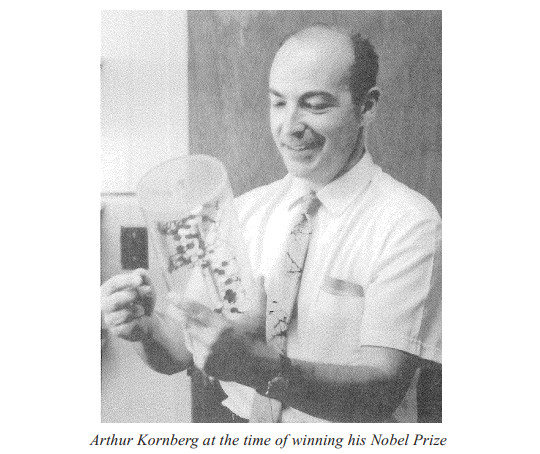
\includegraphics[width=0.75\linewidth]{image/Text5/Fig5.22.png}
\end{figure}

\noindent 63\\
It was and remains a long - standing rule of the Nobel Committee never to split a single prize more than three ways. Had Franklin lived, the problem would have arisen whether to bestow the award upon her or Maurice Wilkins. The Swedes might have resolved the dilemma by awarding them both the Nobel Prize in Chemistry that year. Instead, it went to Max Perutz and John Kendrew, who had elucidated the three - dimensional structures of hemoglobin and myoglobin respectively.\\
一直以来,诺贝尔委员会有个长期不变的规则,即单个奖项的获奖者最多为三人。如果富兰克林还在世,就会出现一个问题,那就是该把这个奖项授予她还是莫里斯·威尔金斯。瑞典人或许会通过在那年同时授予他们诺贝尔化学奖来解决这一困境。然而,该奖项最终授予了马克斯·佩鲁茨和约翰·肯德鲁,他们分别阐明了血红蛋白和肌红蛋白的三维结构。 \\

\noindent 64\\
The discovery of the double helix sounded the death knell for vitalism. Serious scientists, even those religiously inclined, realized that a complete understanding of life would not require the revelation of new laws of nature. Life was just a matter of physics and chemistry, albeit exquisitely organized physics and chemistry. The immediate task ahead would be to figure out how the DNA-encoded script of life went about its work. How does the molecular machinery of cells read the messages of DNA molecules? As the next chapter will reveal, the unexpected complexity of the reading mechanism led to profound insights into how life first came about.\\
DNA双螺旋结构的发现敲响了活力论的丧钟。严谨的科学家,甚至是那些有宗教信仰倾向的科学家,都意识到,要全面理解生命,并不需要揭示新的自然法则。生命仅仅是物理学和化学的问题,尽管是高度有序的物理学和化学。接下来迫在眉睫的任务是弄清楚,由DNA编码的生命 “剧本” 是如何发挥作用的。细胞的分子机制是如何读取DNA分子携带的信息的呢?下一章将会讲到,这一读取机制出乎意料的复杂性,让我们对生命的起源有了深刻的认识。 \\

\newpage

\end{document}